\documentclass[../master]{subfiles}

%\graphicspath{{../eps/}}

\begin{document}

\chapter{シミュレーションによるトラックの再現}
\label{chap::simulation}
\section{\texorpdfstring{$\alpha$}{alpha}線源を用いた測定}
\ref{sec::detection_gas_candidate}節で考えた各検出ガスについて,
実際に$\alpha$線源から放出される$\alpha$粒子のトラックを測定した.
また,それらのデータから各ガスにおけるドリフト速度,ガスの電子増幅率,トラックの幅を決定した.
測定には${}^{241}{\rm Am}$の$\alpha$線源を用いた.
図\ref{fig::a_source_track}に$\alpha$線源のトラックの一例を示す.
図\ref{fig::a_source_track}では検出ガスに\SI{100}{\hecto\pascal}の\isoButaneHydro を用いた.
\ref{sec::detection_gas_candidate}節では6種類の候補を考えたが,
ここからは単体のiso-$\rm C_{4}H_{10}$を除いた5種類について考えていく.
これは単体の\isoButane を検出ガスに用いた場合に,
拡散係数が大きくトラックが太くなると予測されることと,
圧力が\SI{15}{\hecto\pascal}と低く安定したTPC の動作が難しいと予測されるためである.
\begin{figure}
  \centering
  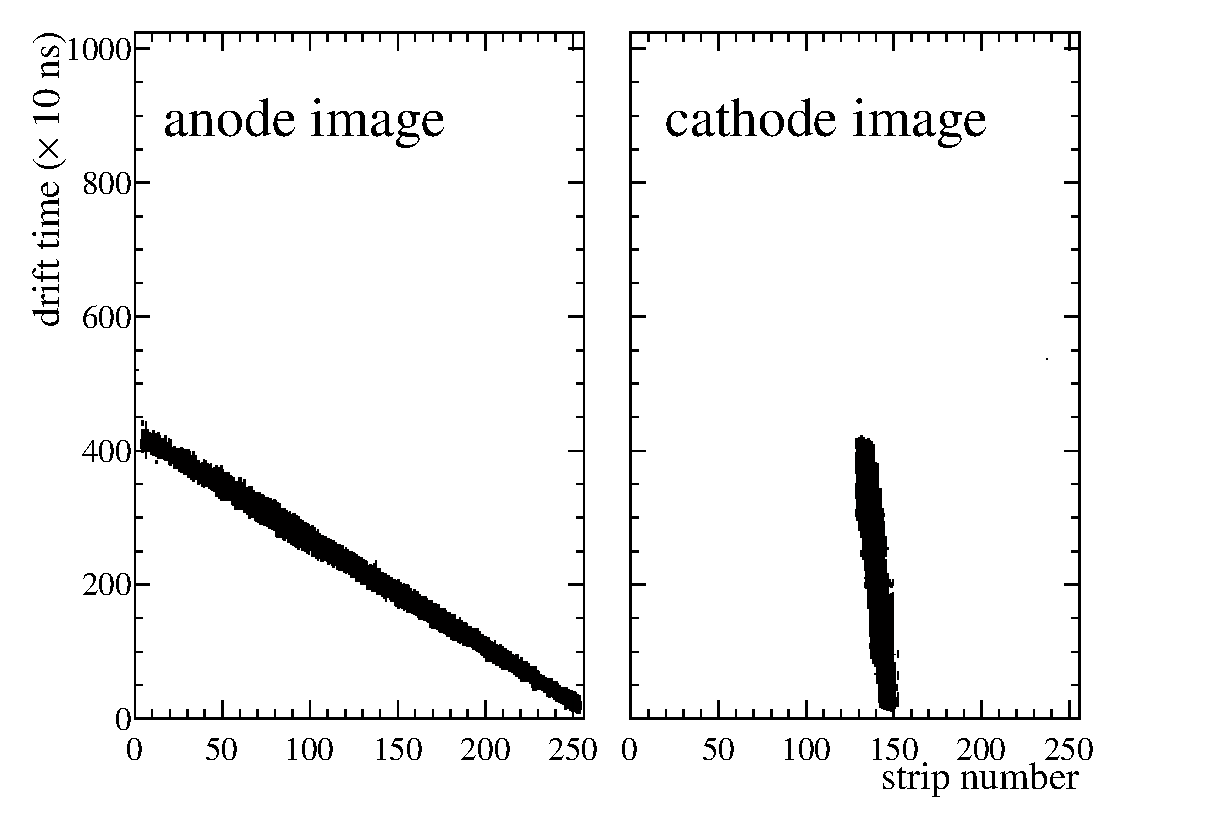
\includegraphics[clip, width=0.9\columnwidth]{0210_7.eps}
  \caption[$\alpha$粒子を測定したトラックの一例.]
          {$\alpha$粒子を測定したトラックの一例.
          検出ガスには\isoButaneHydro を用いた.}
  \label{fig::a_source_track}
\end{figure}

\subsection{ドリフト速度の測定}
電子のドリフト速度を線源によって得られるトラックから実測する.
測定には図\ref{pic::alpha_collimator}のような線源コリメータを用いる.
このコリメータはアクリルで作られており,1つの\ang{0}と4つの\ang{30}の穴が設けられている.
このコリメータを用いることで$\alpha$線の放出方向を\ang{0}と\ang{30}の方向に限定することができる.
\ang{30}方向の$\alpha$線は図\ref{fig::drift_v_image}の右のようにドリフト方向に$\Delta y$~\si{\milli\metre},
それと垂直な方向に$\Delta z$~\si{\milli\metre}移動するとき,
\begin{equation}
  \Delta y = \tan(\ang{30})\times\Delta z \label{eq::deltay_deltaz}
\end{equation}
となる.
MAIKo TPC で取得したトラックの横方向の変分を$\Delta strip$,縦方向の変分を$\Delta t$~\si{\nano\second},
ドリフト速度を$v_{\text{drift}}$~\si{\milli\metre\per\nano\second}とすると,
\begin{align}
  \frac{\Delta z}{\SI{0.4}{\milli\metre}} & = \Delta strip \label{eq::deltaz}\\
  \frac{\Delta y}{v_{\text{drift}}} & = \Delta t \label{eq::deltay}
\end{align}
という関係にある.
式\eqref{eq::deltay_deltaz}, \eqref{eq::deltaz}, \eqref{eq::deltay} より
\begin{equation}
  v_{\text{drift}} = \frac{\tan(\ang{30})\times\Delta strip\times\SI{0.4}{\milli\metre}}{\Delta t}
\end{equation}
とドリフト速度が決定される.
\begin{figure}
  \centering
  \begin{subfigure}{0.45\columnwidth}
    \centering
    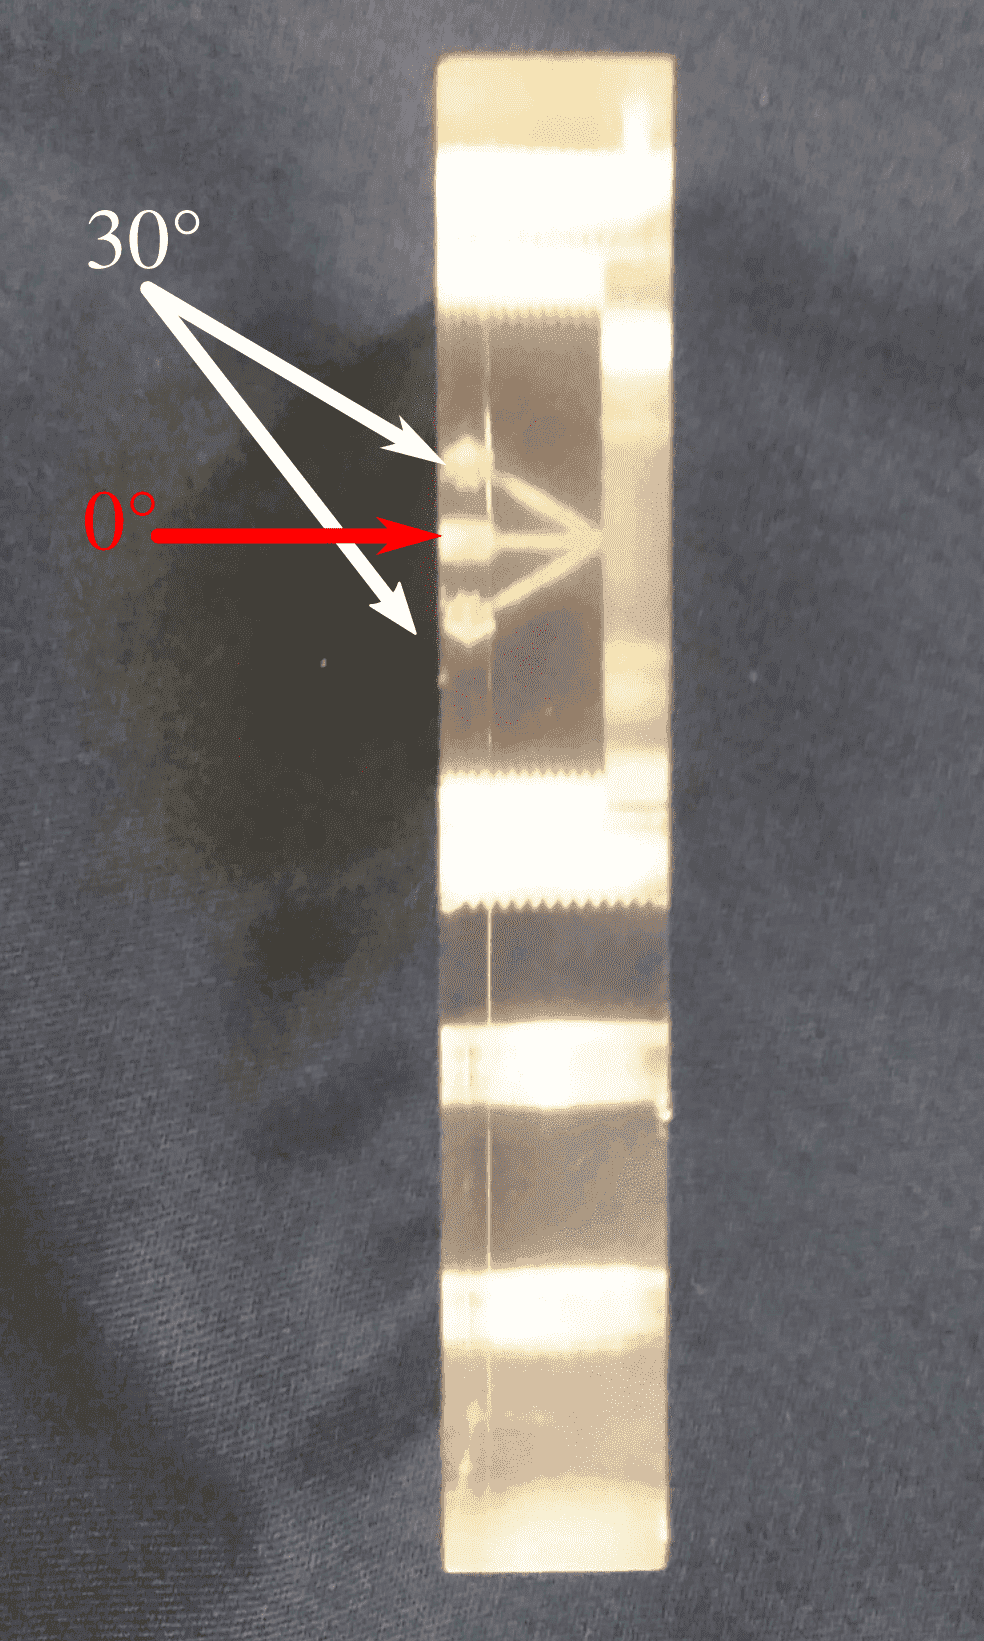
\includegraphics[clip, width=0.8\columnwidth]{image30580-min.png}
    \caption{側面.}
  \end{subfigure}
  \begin{subfigure}{0.45\columnwidth}
    \centering
    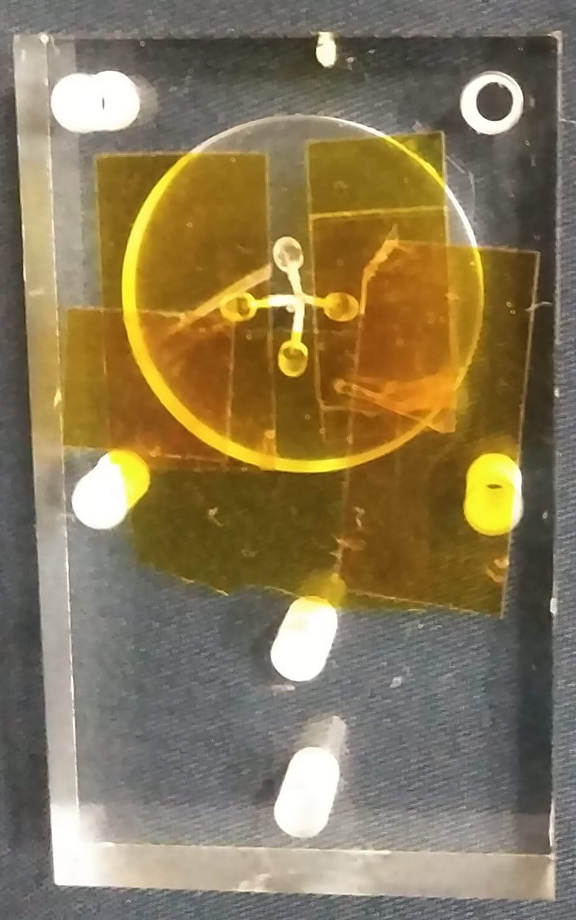
\includegraphics[clip, width=0.8\columnwidth]{IMG_20191225_183542_clip.jpg}
    \caption{正面.}
  \end{subfigure}
  \caption[線源コリメータ.]
          {線源コリメータ.中央に\ang{0},上下左右に\ang{30}の穴が設けられている.
            \ang{0}の穴と1つの\ang{30}の穴を除いてカプトンテープで封じることにより,
            $\alpha$先の放出方向を限定している.
          }
          \label{pic::alpha_collimator}
\end{figure}
\begin{figure}
  \centering
  \begin{minipage}{0.45\columnwidth}
    \centering
    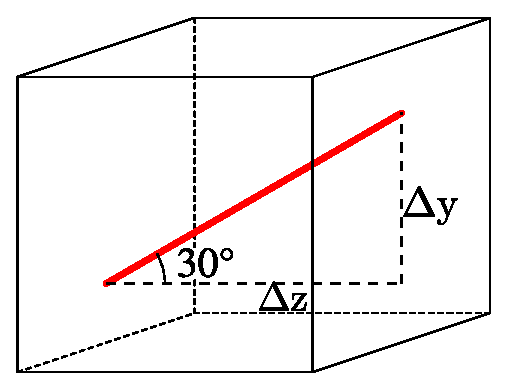
\includegraphics[clip, width=0.9\columnwidth]{drift_v_source.eps}
  \end{minipage}
  \begin{minipage}{0.45\columnwidth}
    \centering
    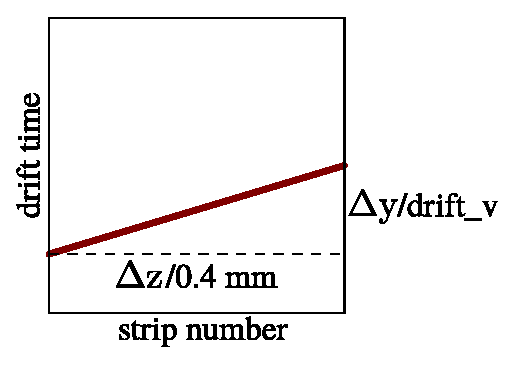
\includegraphics[clip, width=\columnwidth]{drift_v_image.eps}
  \end{minipage}
  \caption[\ang{30}に方向を限定した$\alpha$線と取得される画像データのイメージ.]
          {\ang{30}に方向を限定した$\alpha$線 (左) と取得される画像データ (右) のイメージ.}
  \label{fig::drift_v_image}
\end{figure}

$\alpha$線源を用いて測定したドリフト速度とMagboltz で計算した値を
表\ref{tab::drift_speed_compare}に示す.
$\alpha$線源を用いて測定したドリフト速度と Magboltz を用いて計算したドリフト速度が概ね一致していることが分かる.
ここで,Magboltz の計算値が\SI{0.014}{\milli\metre\per\nano\second}となっていないのは,
MAIKo TPC の実際の運用を簡単にするために設定電圧を切りの良い値にしたためである.
\Methane は実測とMagboltz による計算値に不一致が見られるが,
\Methane のみ\SI{50}{\hecto\pascal} とその他のガスと比較して圧力が半分であるため,
不純物,特に水分の影響を強く受けていると考えられる.
水分のドリフト速度へ与える影響は付録\ref{app::drift_speed_humid_dep}で述べる.
\begin{table}
  \centering
  \caption{実測したドリフト速度とMagboltz を用いて計算したドリフト速度の比較.}
  \label{tab::drift_speed_compare}
  \begin{tabular}{cccc}
    \toprule
    gas & ドリフト電場 (\si{\volt\per\milli\metre}) & 実測値 (\si{\milli\metre\per\nano\second})
    & 計算値 (\si{\milli\metre/\nano\second})\\
    \midrule
    \Methane & 0.429 & 0.0126 & 0.0145 \\
    \MethaneHydro & 4.32 & 0.0140 & 0.0140 \\
    \MethaneHerium & 1.89 & 0.0135 & 0.0140 \\
    \isoButaneHydro & 6.82 & 0.0137 & 0.0140 \\
    \isoButaneHerium & 3.29 & 0.0139 & 0.0141 \\
    \bottomrule
  \end{tabular}
\end{table}
%\begin{figure}
%  \centering
%  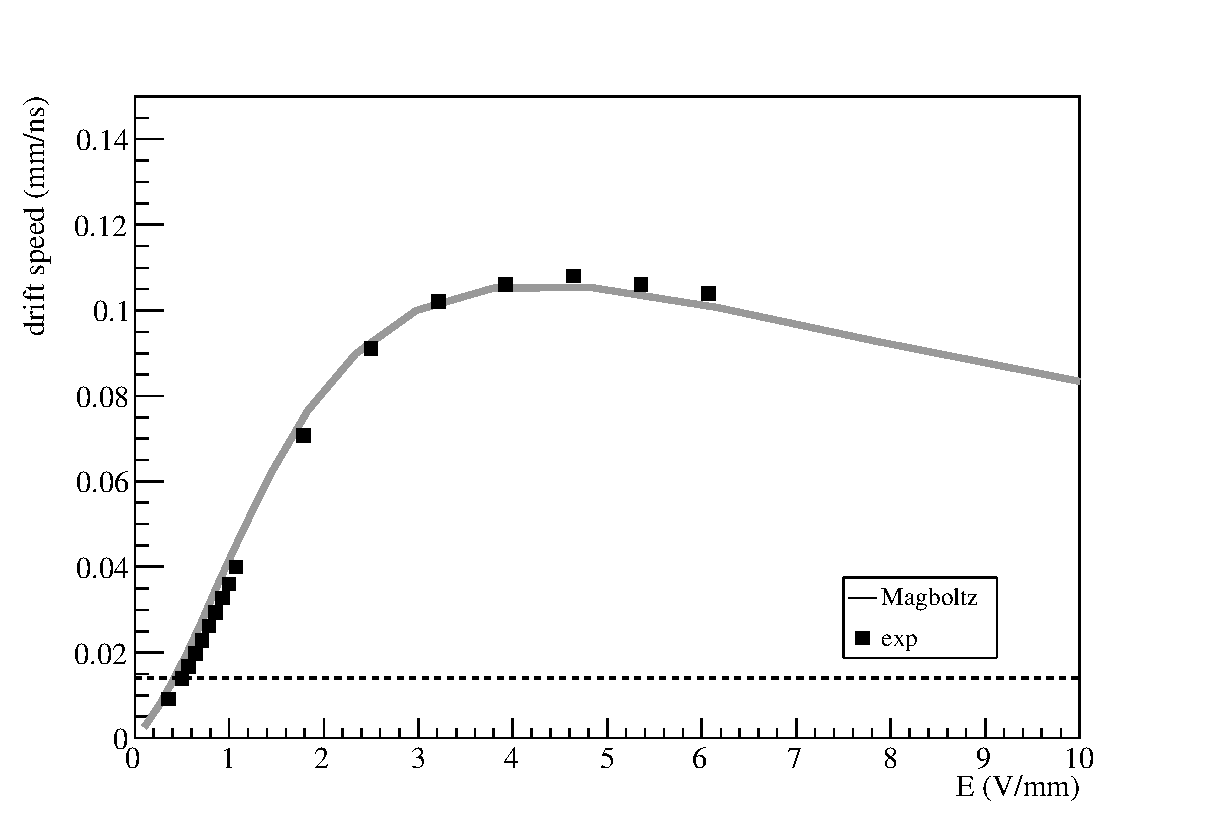
\includegraphics[clip, width=0.9\columnwidth]{drift_v_CH4.eps}
%  \caption[検出ガスに${\rm CH_{4}}$を用いたときのドリフトスピードの電場依存性.]
%          {検出ガスに${\rm CH_{4}}$を用いたときのドリフトスピードの電場依存性.
%            図中の点線は0.014 mm/ns を示す.}
%  \label{fig::drift_v_CH4}
%%  \includegraphics[clip, width=0.7\columnwidth]{drift_v_CH4_H2.eps}
%  \caption{}
%  \label{fig::drift_v_CH4_H2}
%%  \includegraphics[clip, width=0.7\columnwidth]{drift_v_CH4_He.eps}
%  \caption{}
%  \label{fig::drift_v_CH4_He}
%  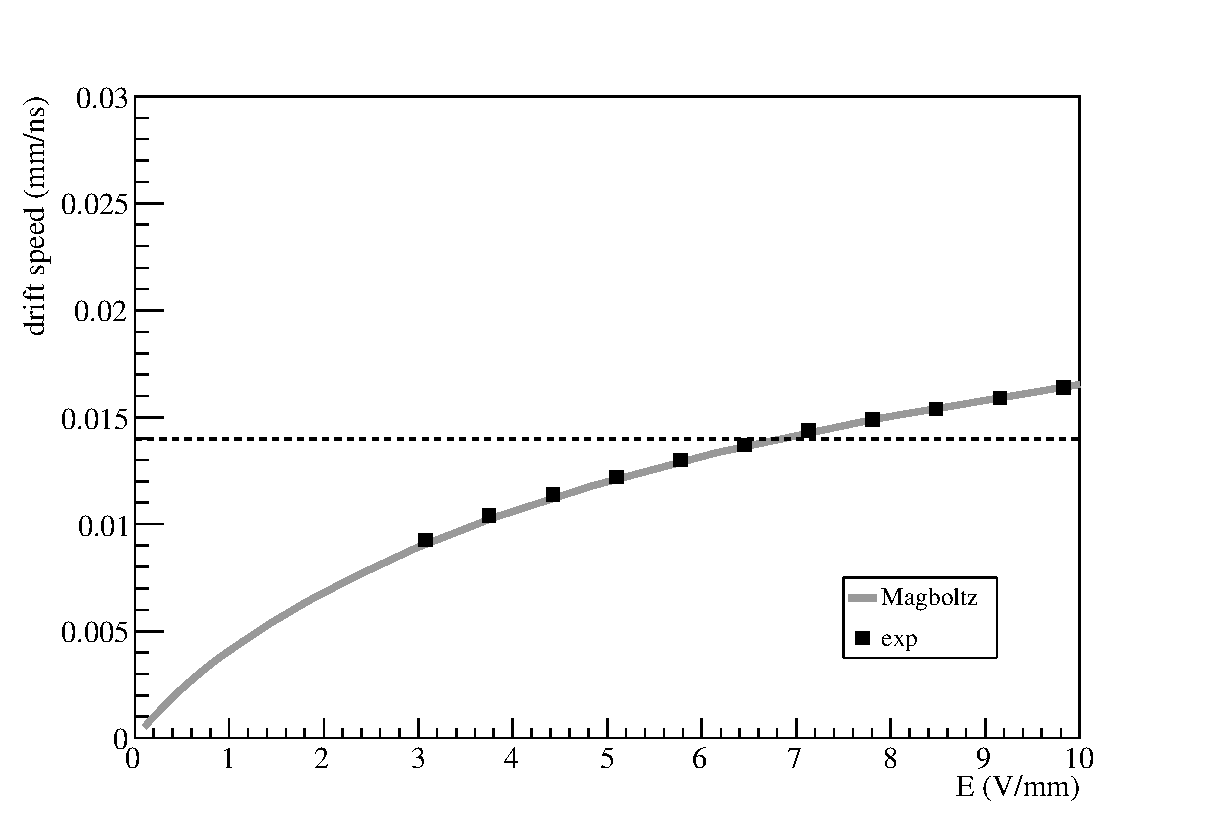
\includegraphics[clip, width=0.9\columnwidth]{drift_v_iC4H10_H2.eps}
%  \caption[検出ガスにiso-${\rm C_{4}H_{10}}$を用いたときのドリフトスピードの電場依存性.]
%          {検出ガスにiso-${\rm C_{4}H_{10}}$を用いたときのドリフトスピードの電場依存性.
%        p    図中の点線は0.014 mm/ns を示す.}
%  \label{fig::drift_v_iC4H10_H2}
%%  \includegraphics[clip, width=0.7\columnwidth]{drift_v_iC4H10_He.eps}
%  \caption{}
%  \label{fig::drift_v_iC4H10_He}
%\end{figure}

\subsection{電子増幅率}
%各部の電圧に対する電子増幅率の依存性を測定した.
GEM および$\mu$-PICによる電子の増幅率を測定した.
増幅率は荷電粒子が検出ガス中を通過した際に発生させた電子数 ($N_{\mathrm{e}}$) と
増幅後に$\mu$-PICによって収集された電子数 ($N'_{\mathrm{e}}$) から求めることができる.
$N_{\mathrm{e}}$は検出ガス中での荷電粒子のエネルギー損失と検出ガスのW値(1つの電子対の生成に必要なエネルギー)から求める.
$N'_{\mathrm{e}}$は$\mu$-PICで収集した電荷から求める.
%詳しい計算方法について以下で述べる.
%
検出ガス中で荷電粒子がエネルギーを損失すると,W値あたり平均1個の電子を電離する.
そのため,荷電粒子のエネルギー損失をW値で除することで$N_{\mathrm{e}}$が求まる.
各検出ガスにおけるエネルギー損失とW値~\cite{energy_per_ion_pair,pdg}を表\ref{tab::energy_loss_and_W_val}に示す.
本研究ではでは${}^{241}\mathrm{Am}$からの$\alpha$線を用いて測定を行った.
${}^{241}\mathrm{Am}$からは\SI{5.48}{\mega\electronvolt}の$\alpha$線が放出される.
今回の測定に用いた$\alpha$線源は線量を大きくするために,多くの${}^{241}\mathrm{Am}$が線源に含まれている.
そのため,物質厚が大きくなっており,$\alpha$線が放出される前に線源中でエネルギーを損失してしまう.
この線源から出ている$\alpha$粒子の持つエネルギーが平均\SI{4.2}{\mega\electronvolt}であることが過去の測定により確認している.
今回の測定では\ang{0}方向に放出された$\alpha$線を用いて測定した.
エネルギー損失は\SI{4.2}{\mega\electronvolt}の$\alpha$粒子が$\mu$-PIC 32 strip分の
距離 (\SI{12.8}{\milli\metre}) で落とすエネルギーを示している.
この距離で発生した電子が$\mu$-PIC の32 stripsで収集される.
\begin{table}
  \centering
  \caption[検出ガスのW値とエネルギー損失と$N_{\rm e}$.]
          {検出ガスのW値~\cite{energy_per_ion_pair,pdg}とエネルギー損失と$N_{\rm e}$.
          エネルギー損失は\SI{4.2}{\mega\electronvolt}の$\alpha$粒子が
          ガス中を\SI{12.8}{\milli\metre} 進んだ時の値である.}
  \label{tab::energy_loss_and_W_val}
  \begin{tabular}{cccc}
    \toprule
    gas & W値 (\si{\electronvolt}) & energy loss (\si{\kilo\electronvolt}) & $N_{\rm e}$\\
    \midrule
    \Methane         & 29.1 & 56.5 & 1.94$\times 10^{3}$ \\
    \MethaneHydro    & 34.2 & 53.4 & 1.56$\times 10^{3}$ \\
    \MethaneHerium   & 39.2 & 59.3 & 1.51$\times 10^{3}$ \\
%    iso-${\rm C_{4}H_{10}}$                 & 26.0 & 0.0552 & 2.12$\times 10^{3}$ \\
    \isoButaneHydro  & 35.4 & 62.0 & 1.75$\times 10^{3}$ \\
    \isoButaneHerium & 44.0 & 58.0 & 1.32$\times 10^{3}$ \\
    \bottomrule
  \end{tabular}
\end{table}

32 strips まとめた$\mu$-PICからの信号波形は図\ref{fig::FADC_waveform}のようなFADC 情報として取得している.
この信号波形を時間で積分することによって32 strips で収集した電荷量を計算することができる.
$\mu$-PICで取得した電気信号は読み出し回路内部で800倍に増幅され,
FADC の入力インピーダンス\SI{50}{\ohm}で電流値を電圧値に変換して取得している.
よって,式\eqref{eq::N'e}で$\mu$-PICで収集した電荷量を得ることができる.
\si{\elementarycharge}は電気素量である.
\begin{equation}
  N'_{\mathrm{e}} = \frac{\int V (t) dt}{ 50 \times 800 \times \si{\elementarycharge}}
  \label{eq::N'e}
\end{equation}
各検出ガスの増幅率と電子の収集効率を畳み込んだ値を表\ref{tab::multiplying_rate}に示す.
ここでは,GEMと$\mu$-PIC の両方による増幅率となっている.
また,測定時のGEM や$\mu$-PICに印加した電圧を表\ref{tab::high_voltage_config_for_gain_meas}に示す.
\begin{table}
  \centering
  \caption{各検出ガスの電子増幅率.}
  \label{tab::multiplying_rate}
  \begin{tabular}{cc}
    \toprule
    gas & 増幅率 (倍) \\
    \midrule
    \Methane         & 700 \\
    \MethaneHydro    & 354 \\
    \MethaneHerium   & 322 \\
    \isoButaneHydro  & 272 \\
    \isoButaneHerium & 392 \\
    \bottomrule
  \end{tabular}
\end{table}
\begin{table}
  \caption{電子増幅率を測定した際の電圧設定.GEM のうちgrid 側をGEMt,$\mu$-PIC側をGEMbとする.}
  \label{tab::high_voltage_config_for_gain_meas}
  \centering
  \begin{tabular}{cccccc}
    \toprule
    gas & plate (\si{\volt}) & grid (\si{\volt}) & GEMt (\si{\volt}) & GEMb (\si{\volt}) & $\mu$-PIC (\si{\volt}) \\
    \midrule
    \Methane         & $-1370$ & $-1290$ & $-560$ & $-150$ & $175$ \\
    \MethaneHydro    & $-2105$ & $-1500$ & $-620$ & $-250$ & $420$ \\
    \MethaneHerium   & $-1465$ & $-1200$ & $-600$ & $-250$ & $400$ \\
    \isoButaneHydro  & $-2255$ & $-1300$ & $-600$ & $-250$ & $400$ \\
    \isoButaneHerium & $-1430$ & $-970$ & $-600$ & $-250$ & $300$ \\
    \bottomrule
  \end{tabular}
\end{table}

\subsection{トラックの幅}
本実験の目的である3$\alpha$に崩壊するイベントでは観測されるトラックが太いと複数のトラックの区別が難しくなり,
トラックを正しく抽出できなくなる.
そこで,\ang{0}の$\alpha$粒子によるトラックの幅を測定した.
図\ref{fig::track_width}に示すように,
トラックの幅にはanode strip 128~ch目のclock方向の幅を用いる.
このようにして決定したトラックの幅とMagboltz を用いて計算した運動方向に対して垂直方向の拡散係数を%表\ref{tab::track_width},
図\ref{fig::diffusion_compare}に示す.
図\ref{fig::diffusion_compare}から分かるようにトラックの幅と拡散係数には正の相関がある.
拡散係数,トラックの幅ともに\isoButaneHydro が最も小さいことが分かる.
\begin{figure}
  \centering
  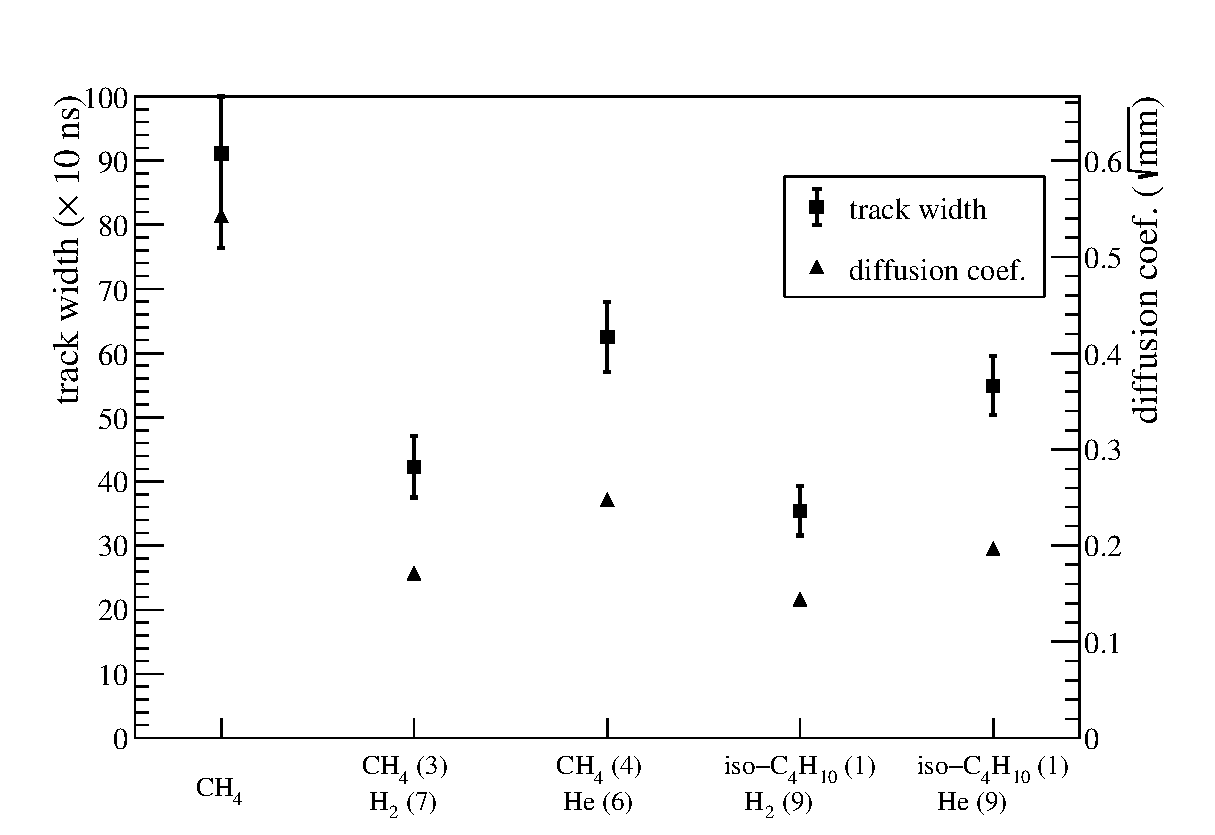
\includegraphics[clip, width=0.5\columnwidth]{track_width.eps}
  \caption{トラックの幅の決定方法のイメージ.
    トラックの幅は有感領域の中央であるanode strip 128~chのclock方向の幅を用いる.}
  \label{fig::track_width}
\end{figure}

%\begin{table}
%  \centering
%  \caption{各検出ガスでのトラックの幅.}
%  \label{tab::track_width}
%  \begin{tabular}{cc}
%    \toprule
%    gas & トラックの幅 ($\times \SI{10}{\nano\second}$)\\
%    \midrule
%    \Methane         & 91.1 \\
%    \MethaneHydro    & 42.3 \\
%    \MethaneHerium   & 62.5 \\
%    \isoButaneHydro  & 35.4 \\
%    \isoButaneHerium & 54.9 \\
%    \bottomrule
%  \end{tabular}
%\end{table}
\begin{figure}
  \centering
  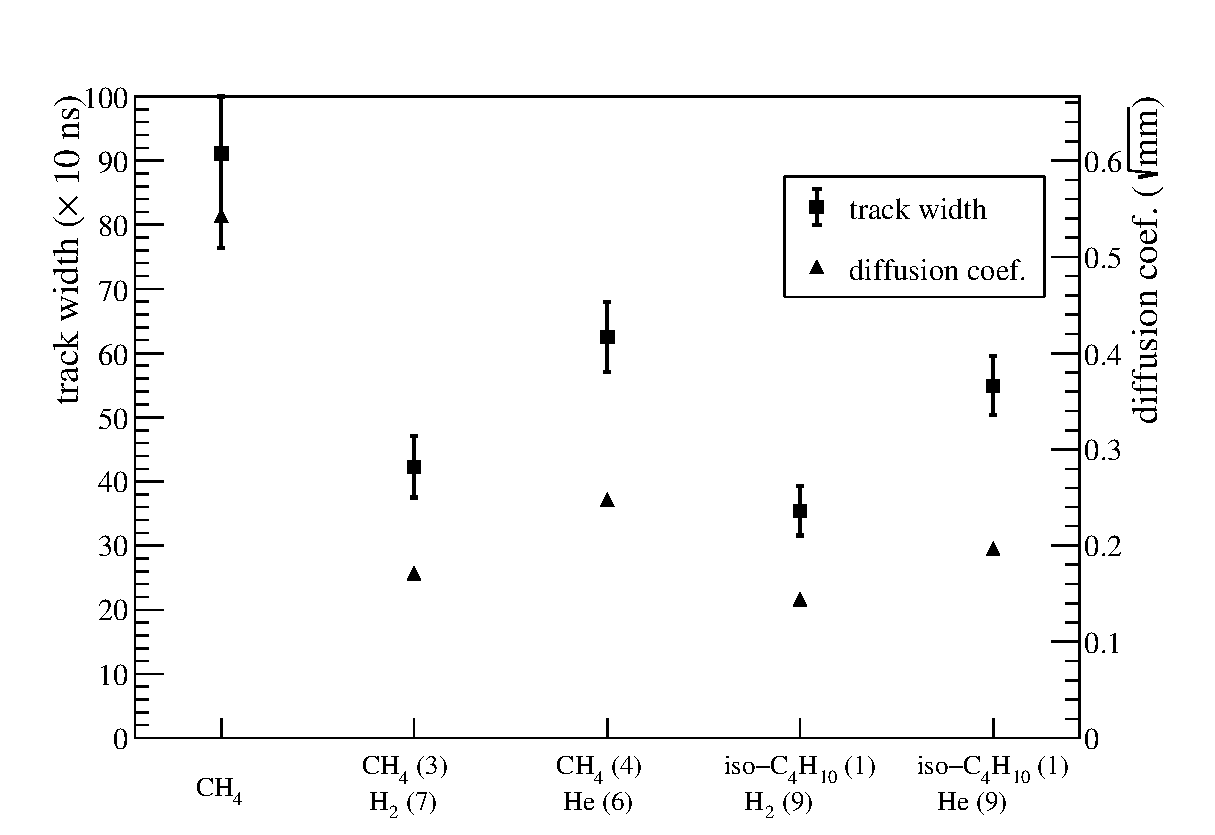
\includegraphics[clip, width=0.9\columnwidth]{diffusion_compare.eps}
  \caption{Magboltz で計算した拡散係数と実測によるトラックの幅.}
  \label{fig::diffusion_compare}
\end{figure}

\section{シミュレーションによる線源データの再現}
MAIKo TPC から得られるトラックをGarfield++~\cite{garfield++}と
Magboltz~\cite{magboltz},SRIM~\cite{SRIM}を用いたシミュレーションによりMAIKo TPC で測定されるトラックの再現を試みた.
シミュレーションでは,ドリフト電場,W値,電子増幅率,検出ガスの密度を固定した上で,
最もよく測定結果を再現する信号の閾値を探索した.
電子増幅率は$\alpha$線源を用いた測定値を用いた.
シミュレーションは以下の手順%(図\ref{fig::simulation_flow})
で行った.
\begin{enumerate}
\item\label{sim::particle_generate}
  トラックを生成する荷電粒子のエネルギー,運動量を決定し,
  Garfield++のSrimTrack に登録する.
\item
  SrimTrack によりトラックの周囲に電子を生成する.
\item
  電子をMagboltz で求めたドリフト速度と拡散係数に基づき読み出し領域へドリフトさせる.
\item
  電子のドリフト時間を信号処理回路の応答関数で畳み込む.
  すなわち,読み出し領域に到達した電子1つにつき図\ref{fig::mu-pic_readout}に示すような電気信号を
  各strip の信号波形に加算する.
\item
  設定した信号波形の閾値に基づき,信号波形を白黒画像に変換しanode image とcathode image を生成する.
\end{enumerate}
$\alpha$線源を用いた場合のシミュレーションと測定の比較を以下に示す.
図\ref{fig::track_comp_ch4}は\SI{50}{\hecto\pascal}の\Methane におけるトラック,
図\ref{fig::track_comp_ch4_h2}は\SI{100}{\hecto\pascal}の\MethaneHydro におけるトラック,
図\ref{fig::track_comp_ch4_he}は\SI{100}{\hecto\pascal}の\MethaneHerium におけるトラック, 
図\ref{fig::track_comp_ic4h10_h2}は\SI{100}{\hecto\pascal}の\isoButaneHydro におけるトラック,
図\ref{fig::track_comp_ic4h10_he}は\SI{100}{\hecto\pascal}の\isoButaneHerium におけるトラックである.
これらの$\alpha$線は図\ref{fig::drift_v_image}のように有感領域を貫通している.
信号の閾値を\SI{0.1}{\milli\volt}とすると,それぞれの検出ガスでの$\alpha$線源によるトラックを,
シミュレーションで再現できる.
\begin{figure}
  \centering
  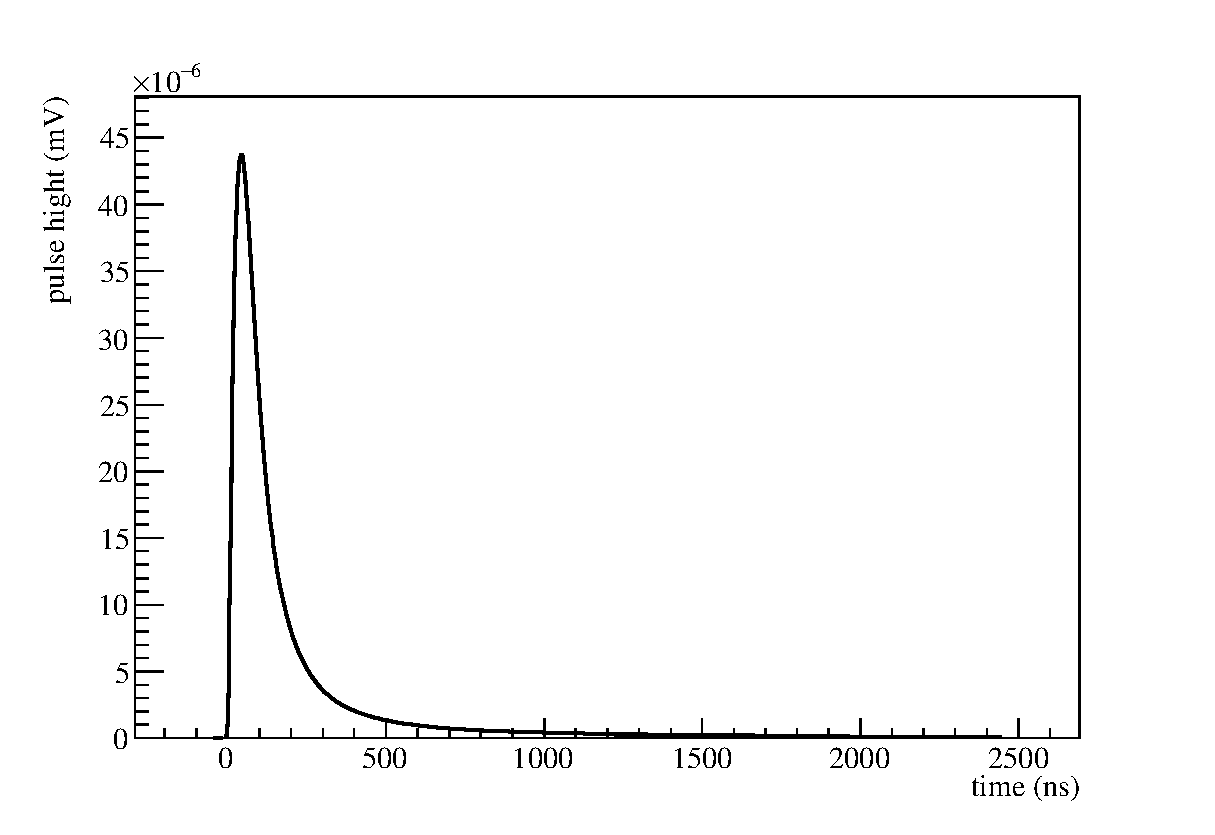
\includegraphics[clip, width=0.9\columnwidth]{waveform.eps}
  \caption{1電子が$\mu$-PICに到達した時に読み出される電気信号.}
  \label{fig::mu-pic_readout}
\end{figure}

\begin{figure}
  \centering
  \begin{subfigure}{0.48\columnwidth}
    \centering
    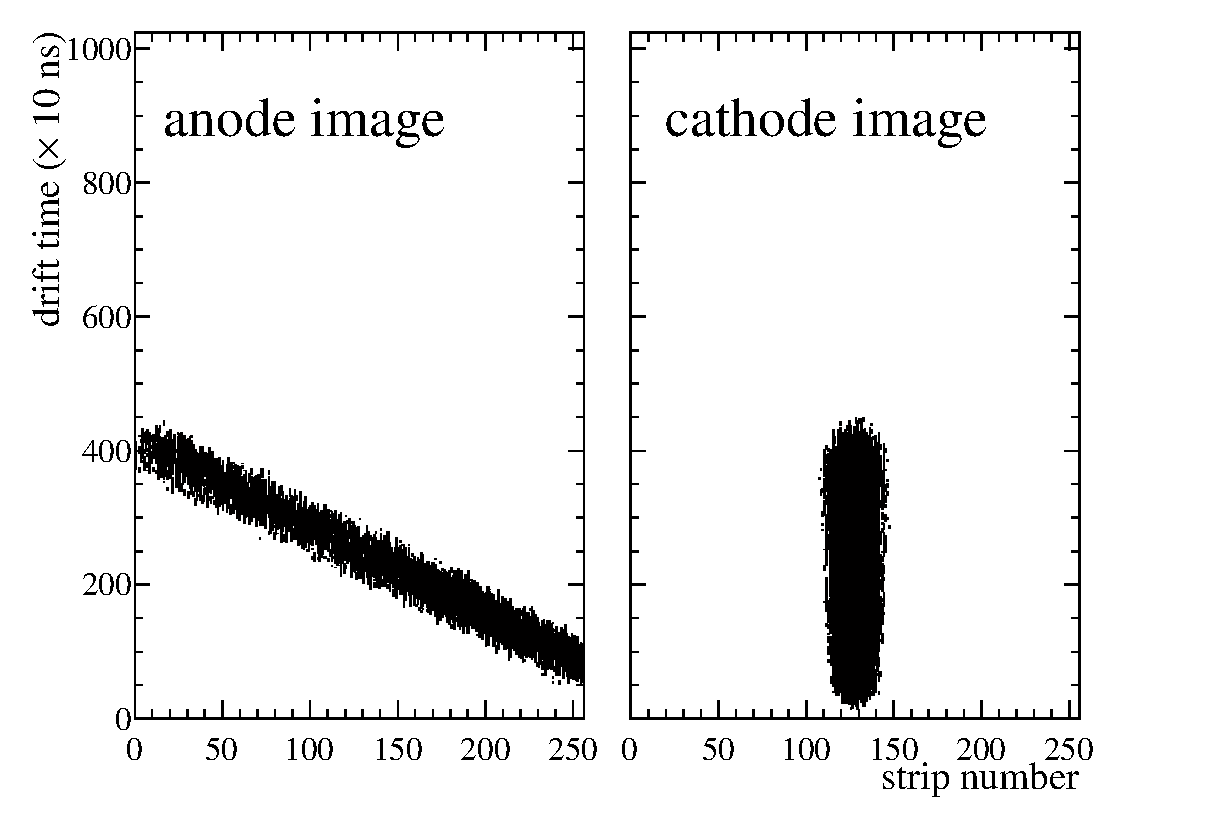
\includegraphics[clip, width=\columnwidth, trim=0 0 50 0]{CH4_0.eps}
    \caption{シミュレーションによるトラック.}
  \end{subfigure}
  \begin{subfigure}{0.48\columnwidth}
    \centering
    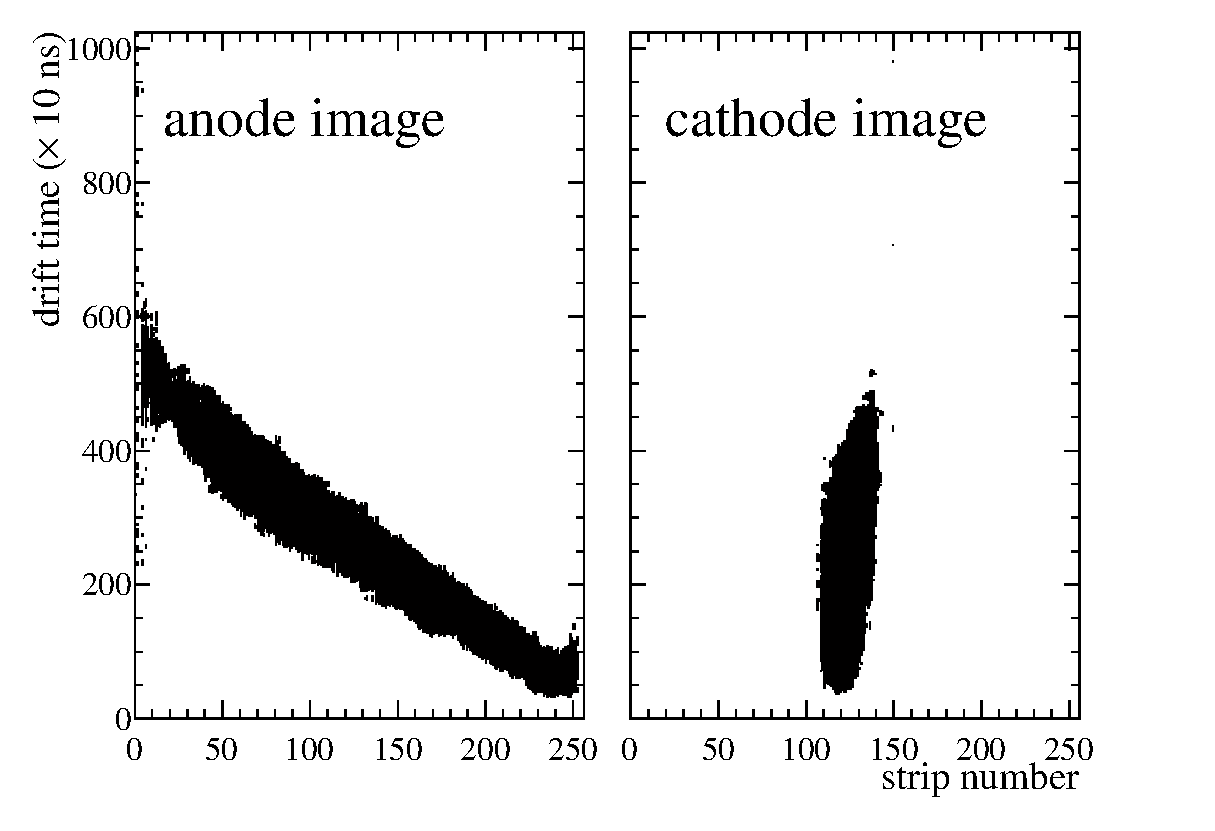
\includegraphics[width=\columnwidth, trim=0 0 50 0]{0160_5.eps}
    \caption{$\alpha$線源によるトラック.}
  \end{subfigure}
  \caption{$\alpha$粒子のトラック(\Methane の場合).}
  \label{fig::track_comp_ch4}
\end{figure}

\begin{figure}
  \centering
  \begin{subfigure}{0.48\columnwidth}
    \centering
    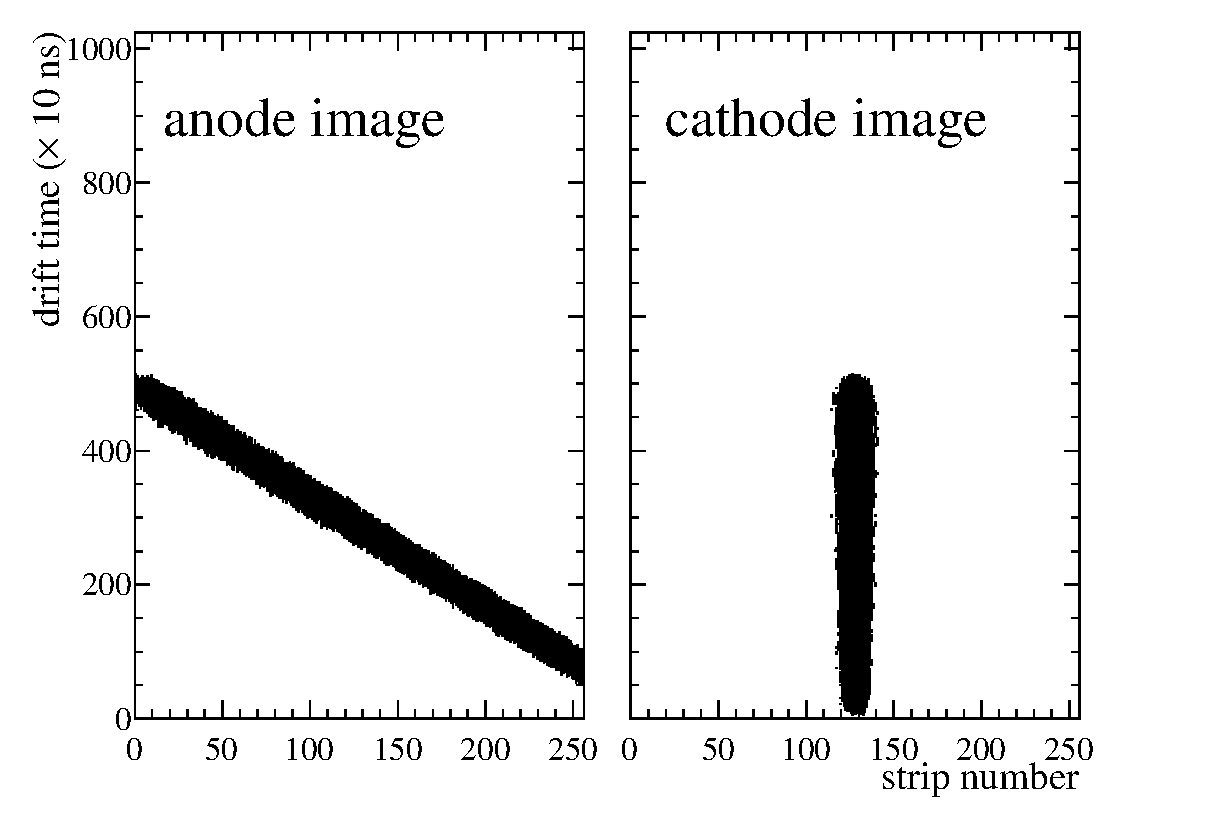
\includegraphics[clip, width=\columnwidth, trim=0 0 50 0]{CH4_3_H2_7_0.eps}
    \caption{シミュレーションによるトラック.}
  \end{subfigure}
  \begin{subfigure}{0.48\columnwidth}
    \centering
    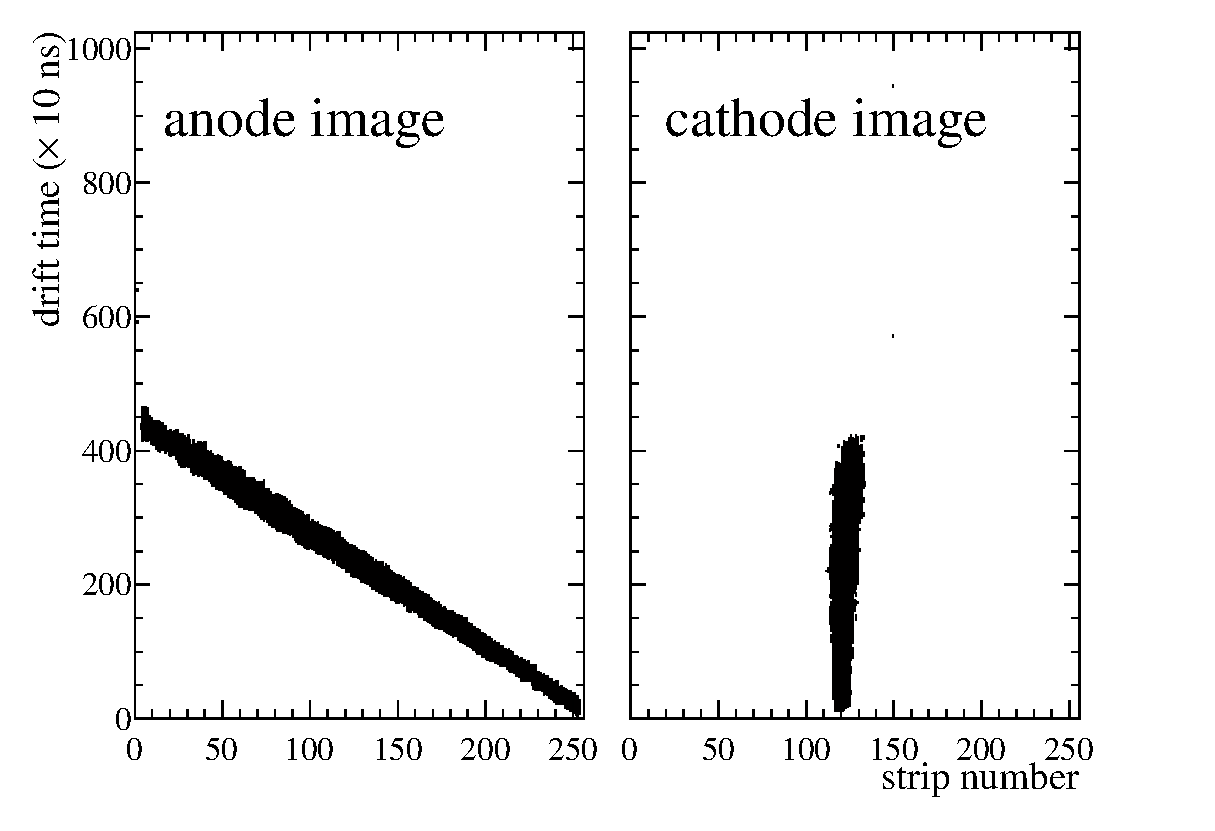
\includegraphics[clip, width=\columnwidth, trim=0 0 50 0]{0207_7.eps}
    \caption{$\alpha$線源によるトラック.}
  \end{subfigure}
  \caption{$\alpha$粒子のトラック(\MethaneHydro の場合).}
  \label{fig::track_comp_ch4_h2}
\end{figure}

\begin{figure}
  \centering
  \begin{subfigure}{0.48\columnwidth}
    \centering
    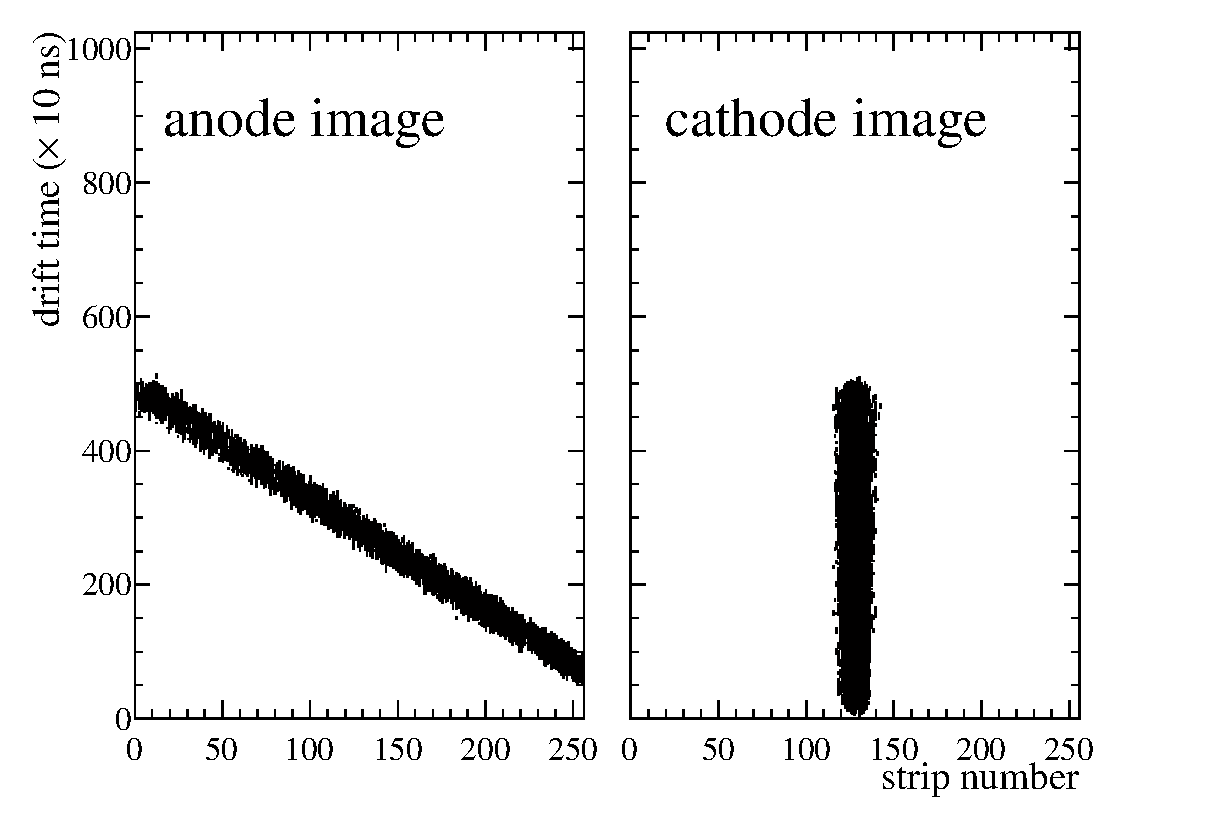
\includegraphics[clip, width=\columnwidth, trim=0 0 50 0]{CH4_4_He_6_0.eps}
    \caption{シミュレーションによるトラック.}
  \end{subfigure}
  \begin{subfigure}{0.48\columnwidth}
    \centering
    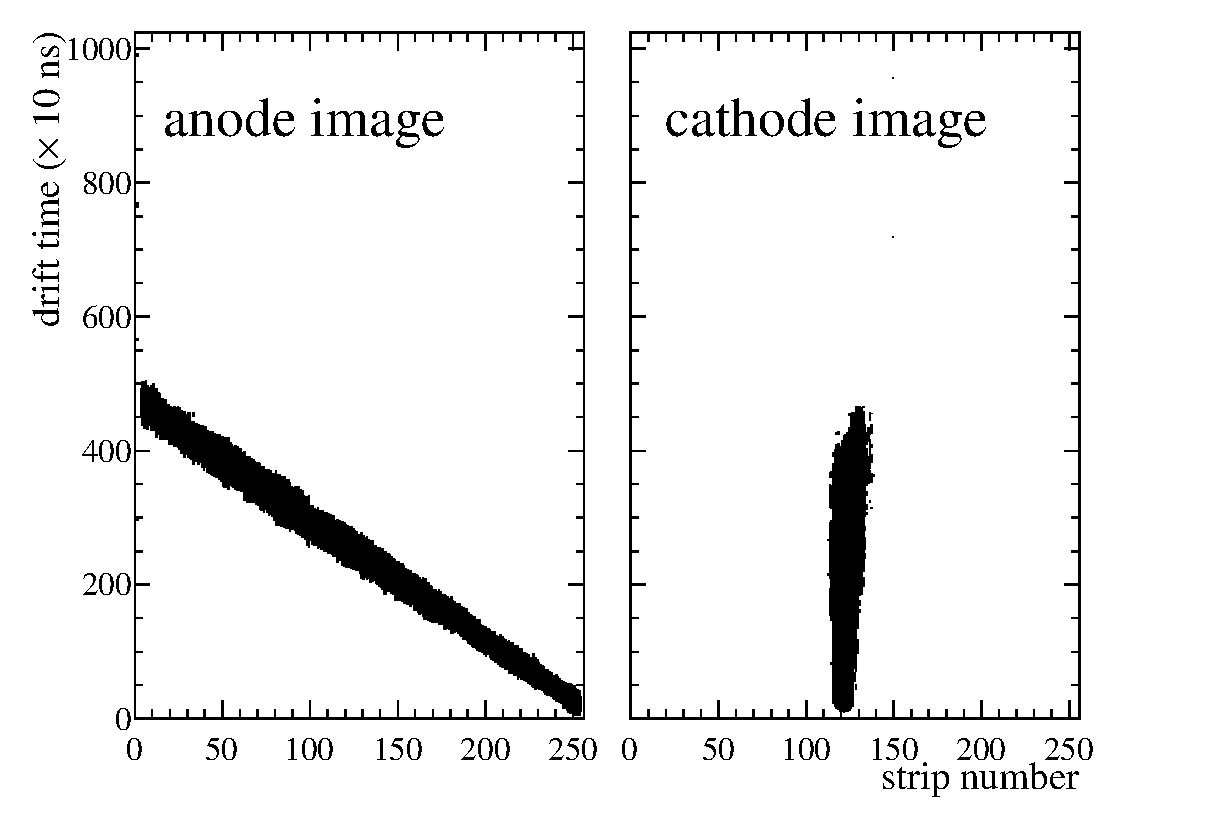
\includegraphics[clip, width=\columnwidth, trim=0 0 50 0]{0163_3.eps}
    \caption{$\alpha$線源によるトラック.}
  \end{subfigure}
  \caption{$\alpha$粒子のトラック [\MethaneHerium の場合].}
  \label{fig::track_comp_ch4_he}
\end{figure}

\begin{figure}
  \centering
  \begin{subfigure}{0.48\columnwidth}
    \centering
    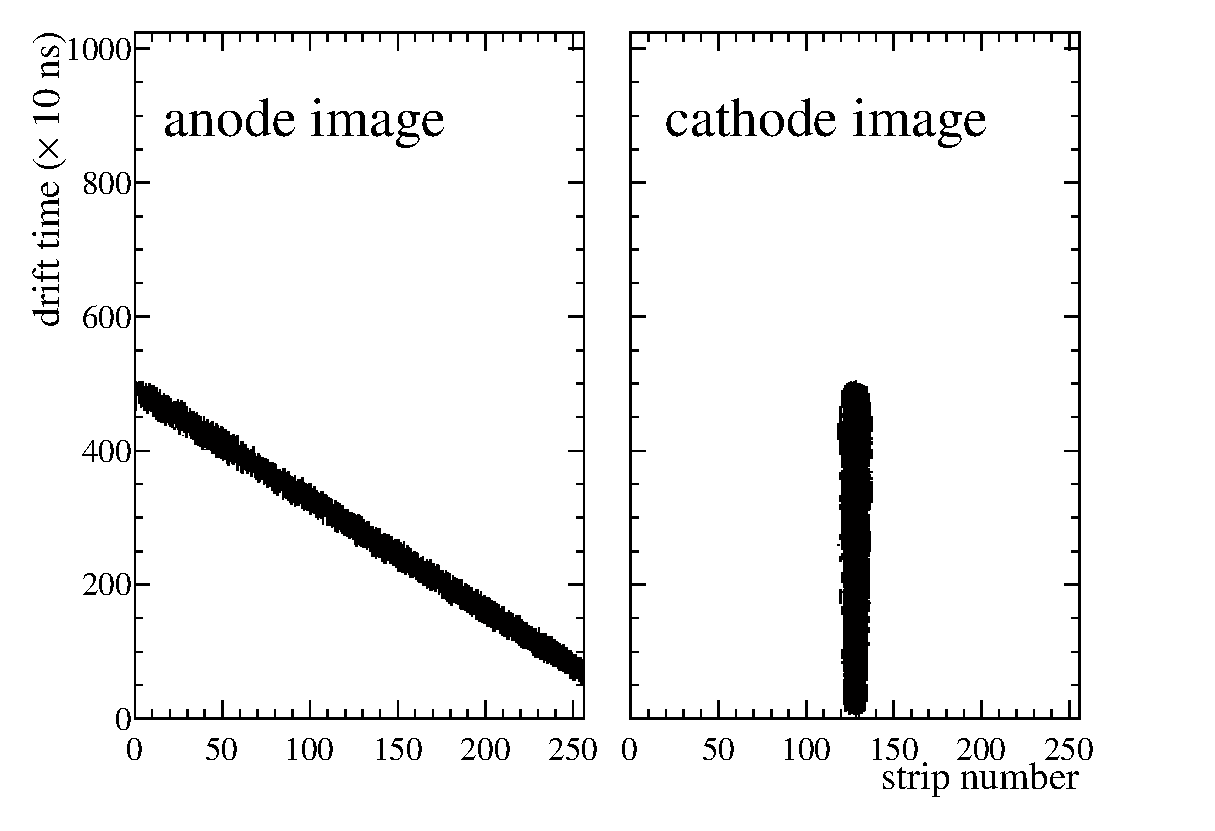
\includegraphics[clip, width=\columnwidth, trim=0 0 50 0]{iC4H10_1_H2_9_0.eps}
    \caption{シミュレーションによるトラック.}
  \end{subfigure}
  \begin{subfigure}{0.48\columnwidth}
    \centering
    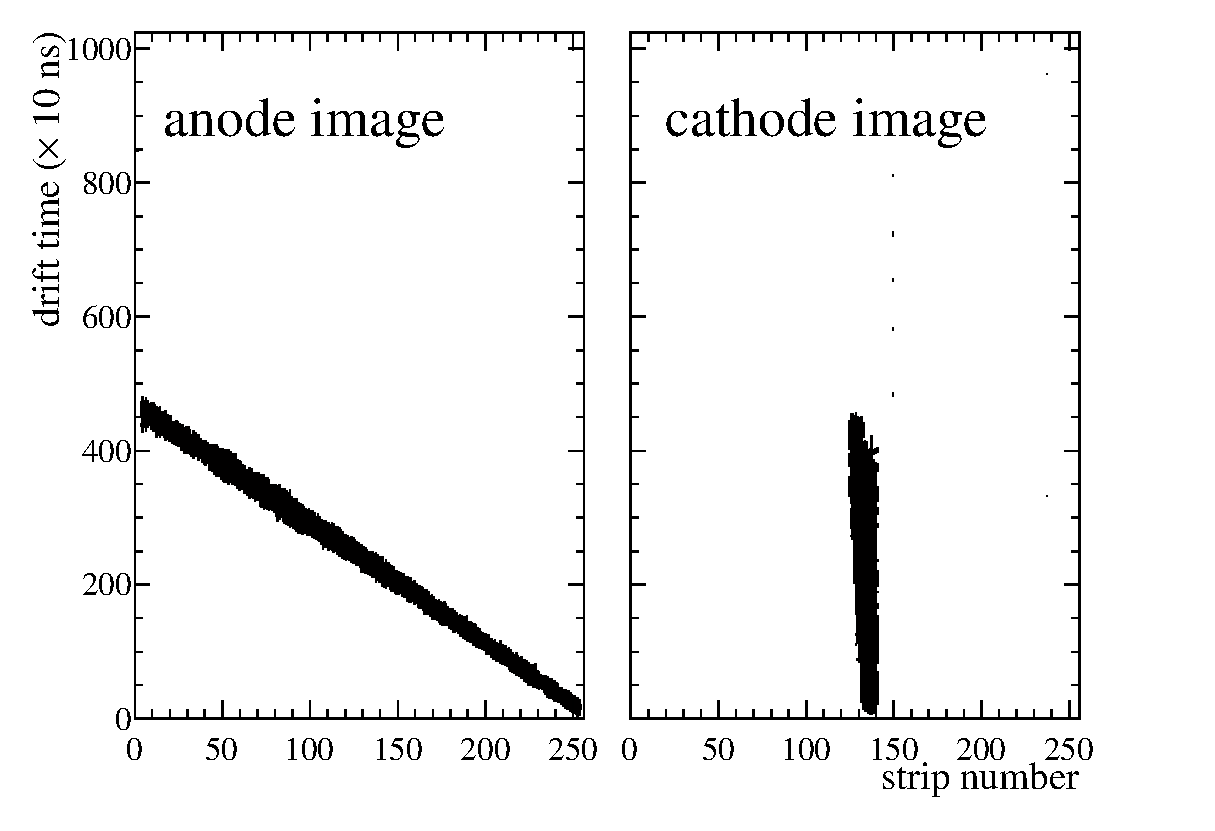
\includegraphics[clip, width=\columnwidth, trim=0 0 50 0]{0210_14.eps}
    \caption{$\alpha$線源によるトラック.}
  \end{subfigure}
  \caption{$\alpha$粒子のトラック [\isoButaneHydro の場合].}
  \label{fig::track_comp_ic4h10_h2}
\end{figure}

\begin{figure}
  \centering
  \begin{subfigure}{0.48\columnwidth}
    \centering
    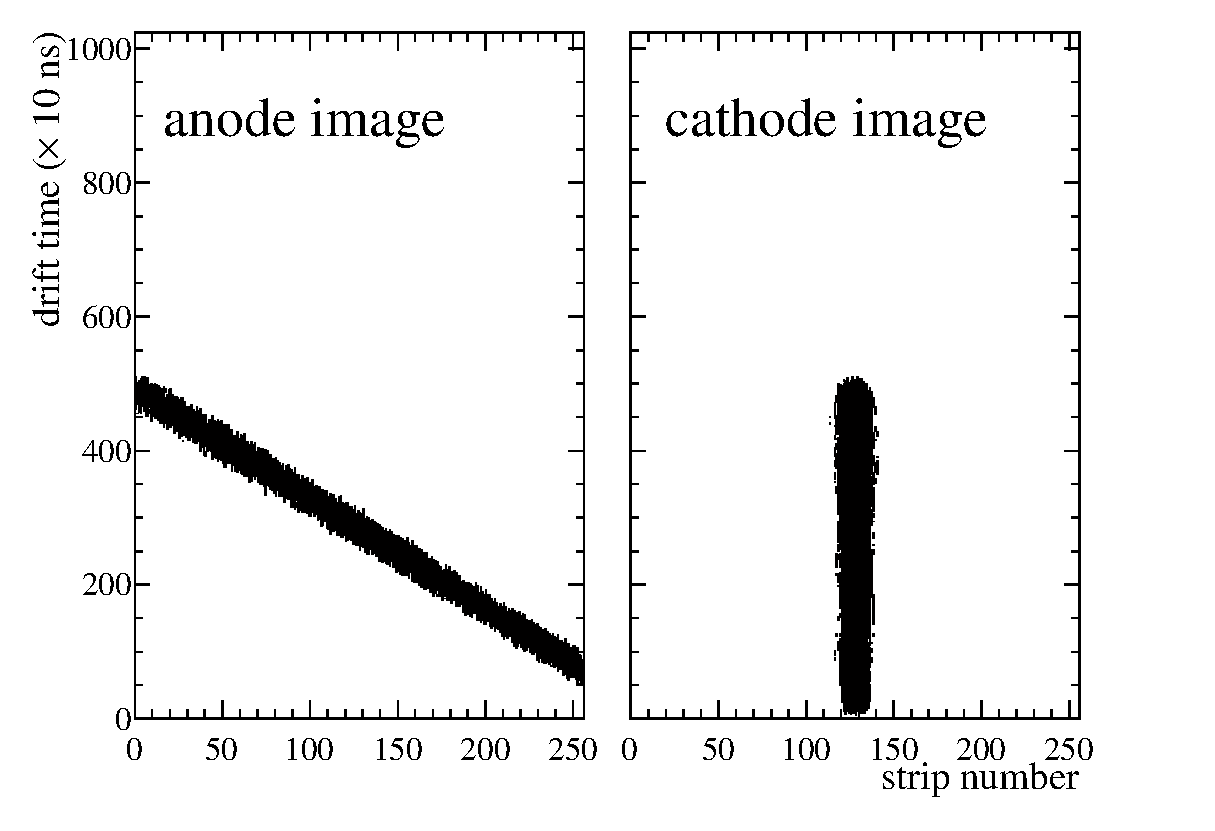
\includegraphics[clip, width=\columnwidth, trim=0 0 50 0]{iC4H10_1_He_9_0.eps}
    \caption{シミュレーションによるトラック.}
  \end{subfigure}
  \begin{subfigure}{0.48\columnwidth}
    \centering
    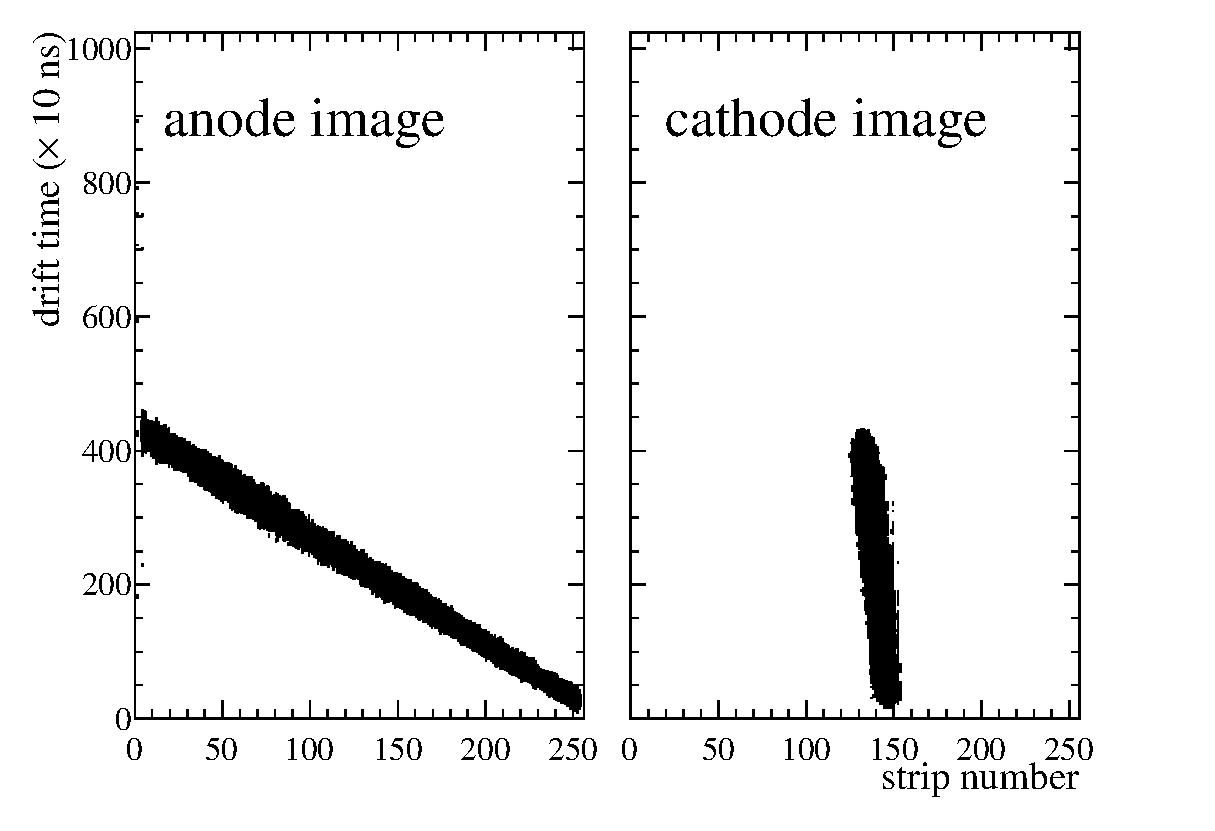
\includegraphics[clip, width=\columnwidth, trim=0 0 50 0]{0176_1.eps}
    \caption{$\alpha$線源によるトラック.}
  \end{subfigure}
  \caption{$\alpha$粒子のトラック [\isoButaneHerium の場合].}
  \label{fig::track_comp_ic4h10_he}
\end{figure}

$\alpha$線源から放出される$\alpha$粒子のエネルギーは平均\SI{4.2}{\mega\electronvolt}である.
一方で,本研究で検出を目指している$0_2^+$状態からの崩壊$\alpha$粒子のエネルギーは数百\si{\kilo\electronvolt}である.
そこで,$\alpha$線源の前に\SI{15}{\micro\metre}のカプトン膜を設置することで$\alpha$粒子のエネルギーを減衰させ,
低エネルギー$\alpha$粒子での測定を行った.
$\alpha$粒子のエネルギーは有感領域と線源の間にある検出ガスによってさらに低下し
TPC の有感領域では約\SI{1}{\mega\electronvolt}となる.
低エネルギー$\alpha$粒子のトラックを
図\ref{fig::track_ch4_loss} [\Methane~(\SI{50}{\hecto\pascal})],
\ref{fig::track_ch4_h2_loss} [\MethaneHydro~(\SI{100}{\hecto\pascal})],
\ref{fig::track_ch4_he_loss} [\MethaneHerium~(\SI{100}{\hecto\pascal})],
\ref{fig::track_ic4h10_h2_loss} [\isoButaneHydro~(\SI{100}{\hecto\pascal})],
\ref{fig::track_ic4h10_he_loss} [\isoButaneHerium~(\SI{100}{\hecto\pascal})] に示す.
コリメータによって$\alpha$線の方向を\ang{30}に制限したため,斜めのトラックとなっている.
シミュレーションでは有感領域の横から\SI{500}{\kilo\electronvolt}の$\alpha$粒子を入射させた.
これらの$\alpha$粒子はMAIKo TPC の有感領域中で停止している.
$\alpha$線源から放出されるエネルギーに広がりがあるため,
エネルギーを完全に一致できていないが,トラックの太さの傾向は再現できている.
\begin{figure}
  \centering
  \begin{subfigure}{0.48\columnwidth}
    \centering
    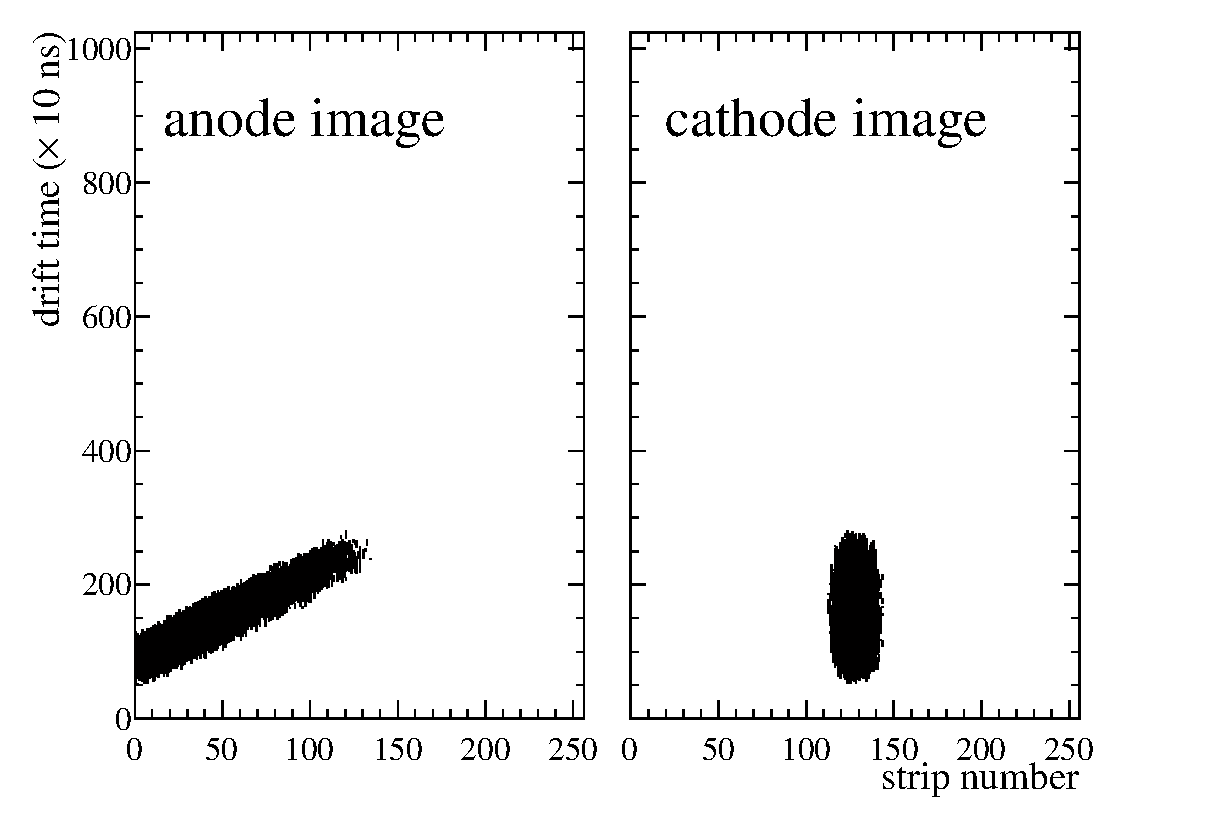
\includegraphics[clip, width=\columnwidth, trim=0 0 50 0]{a_source_CH4_50_nostr_3.eps}
    \caption{シミュレーションによるトラック.}
  \end{subfigure}
  \begin{subfigure}{0.48\columnwidth}
    \centering
    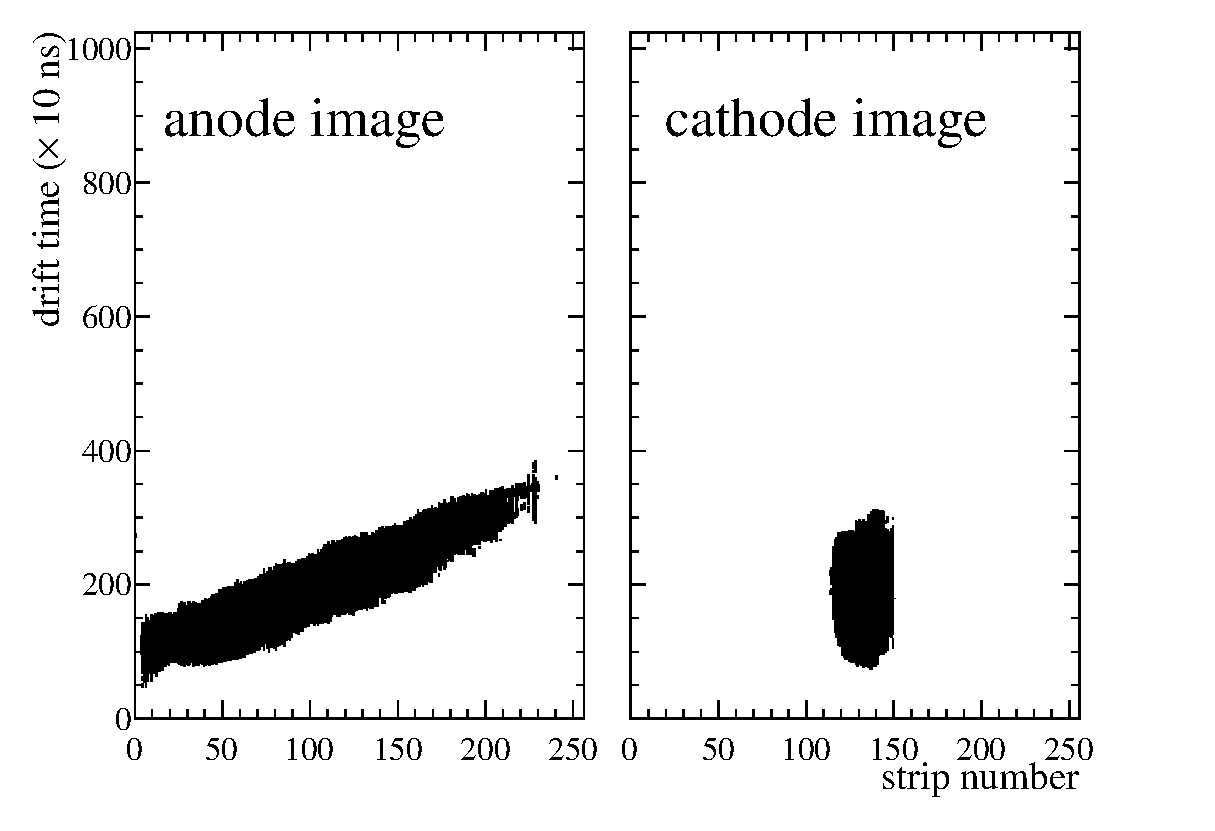
\includegraphics[clip, width=\columnwidth, trim=0 0 50 0]{0146_16.eps}
    \caption{$\alpha$線源によるトラック.}
  \end{subfigure}
  \caption{低エネルギー$\alpha$粒子のトラック [\Methane の場合].}
  \label{fig::track_ch4_loss}
\end{figure}
\begin{figure}
  \centering
  \begin{subfigure}{0.48\columnwidth}
    \centering
    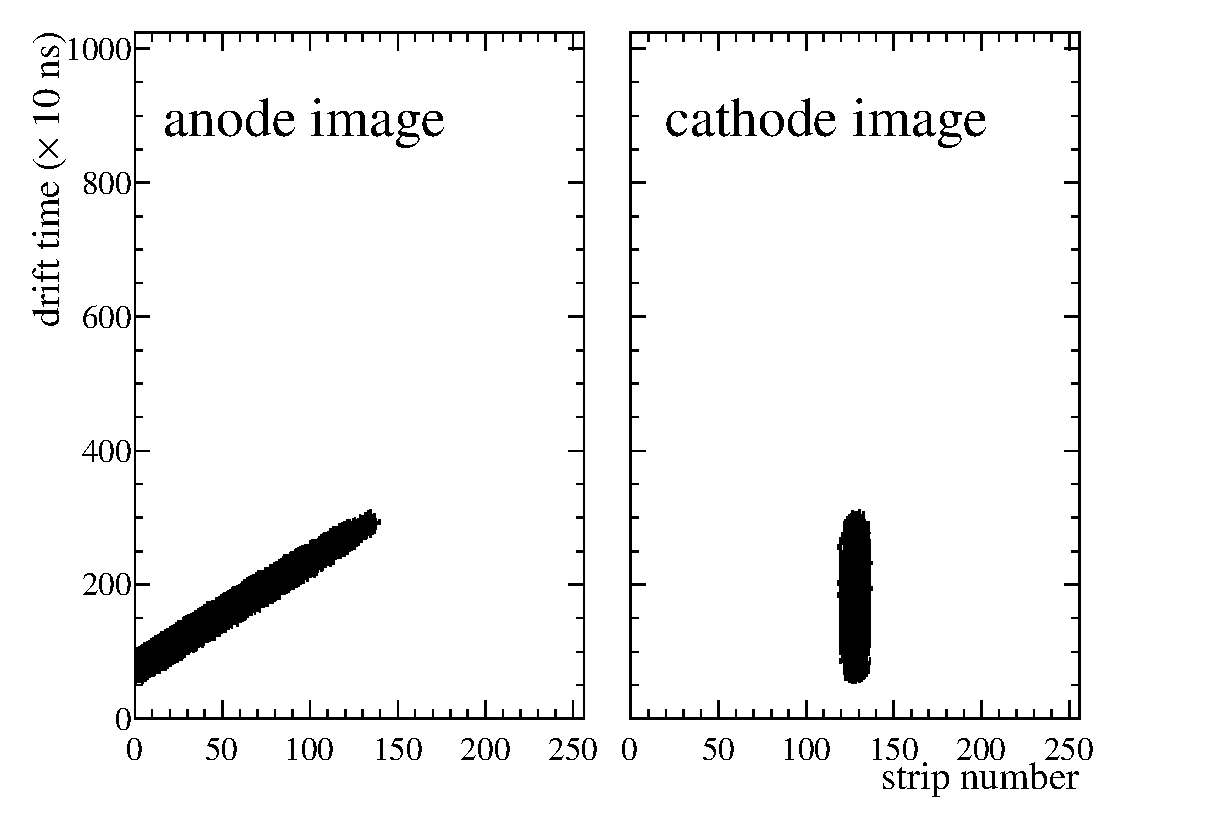
\includegraphics[clip, width=\columnwidth, trim=0 0 50 0]{a_source_CH4_3_H2_7_100_nostr_0.eps}
    \caption{シミュレーションによるトラック.}
  \end{subfigure}
  \begin{subfigure}{0.48\columnwidth}
    \centering
    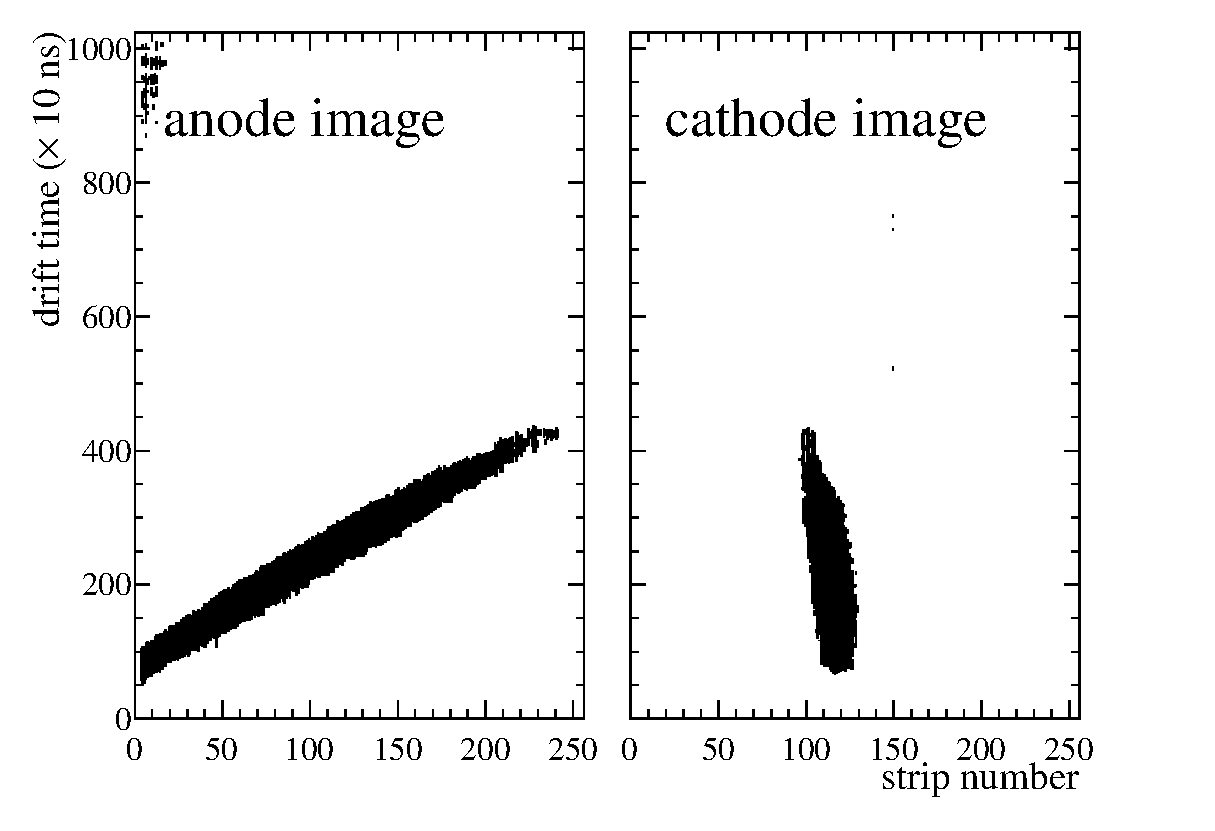
\includegraphics[clip, width=\columnwidth, trim=0 0 50 0]{0209_22.eps}
    \caption{$\alpha$線源によるトラック.}
  \end{subfigure}
  \caption{低エネルギー$\alpha$粒子のトラック [\MethaneHydro の場合].}
  \label{fig::track_ch4_h2_loss}
\end{figure}
\begin{figure}
  \centering
  \begin{subfigure}{0.48\columnwidth}
    \centering
    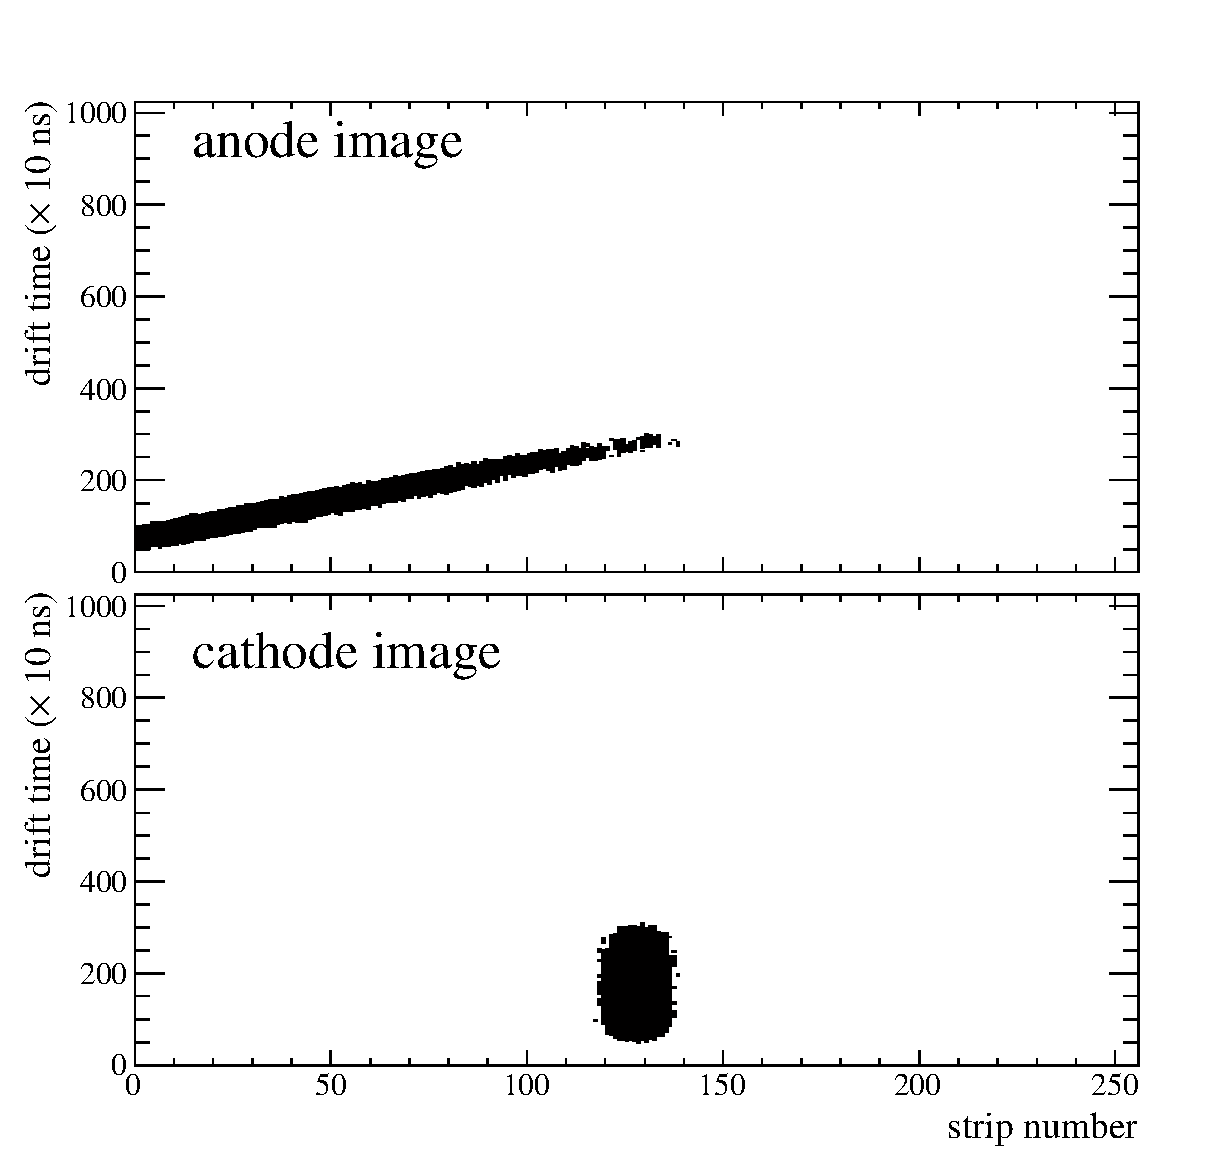
\includegraphics[clip, width=\columnwidth, trim=0 0 50 0]{a_source_CH4_4_He_6_100_nostr_0.eps}
    \caption{シミュレーションによるトラック.}
  \end{subfigure}
  \begin{subfigure}{0.48\columnwidth}
    \centering
    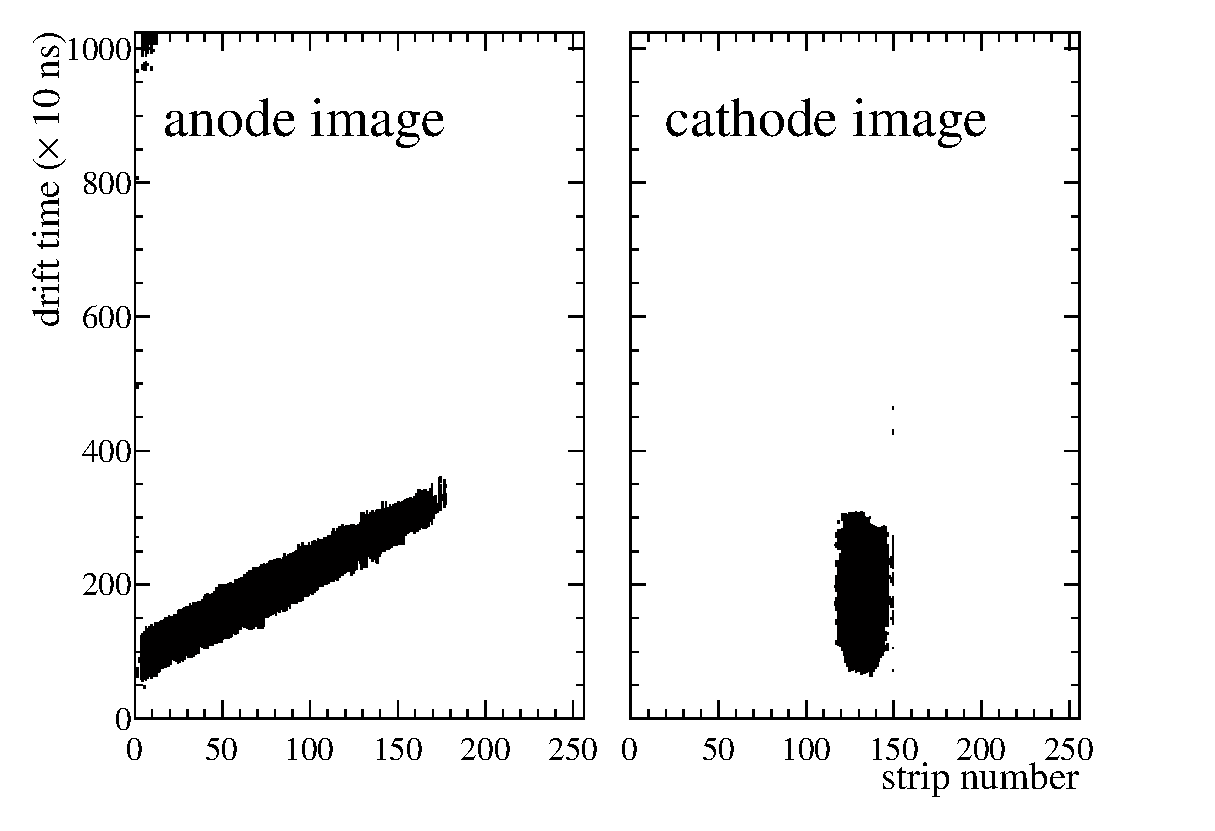
\includegraphics[clip, width=\columnwidth, trim=0 0 50 0]{0204_24.eps}
    \caption{$\alpha$線源によるトラック.}
  \end{subfigure}
  \caption{低エネルギー$\alpha$粒子のトラック [\MethaneHerium の場合].}
  \label{fig::track_ch4_he_loss}
\end{figure}
\begin{figure}
  \centering
  \begin{subfigure}{0.48\columnwidth}
    \centering
    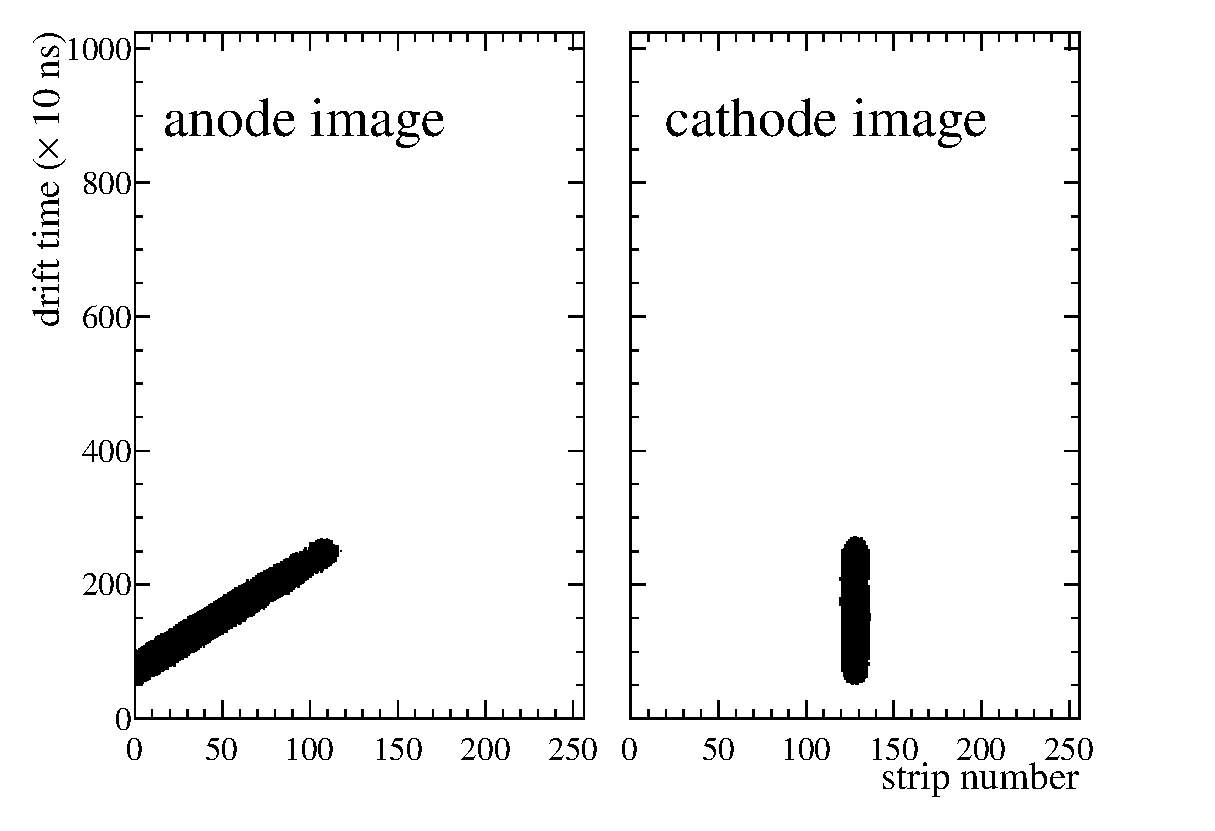
\includegraphics[clip ,width=\columnwidth, trim=0 0 50 0]{a_source_iC4H10_1_H2_9_100_nostr_1.eps}
    \caption{シミュレーションによるトラック.}
  \end{subfigure}
  \begin{subfigure}{0.48\columnwidth}
    \centering
    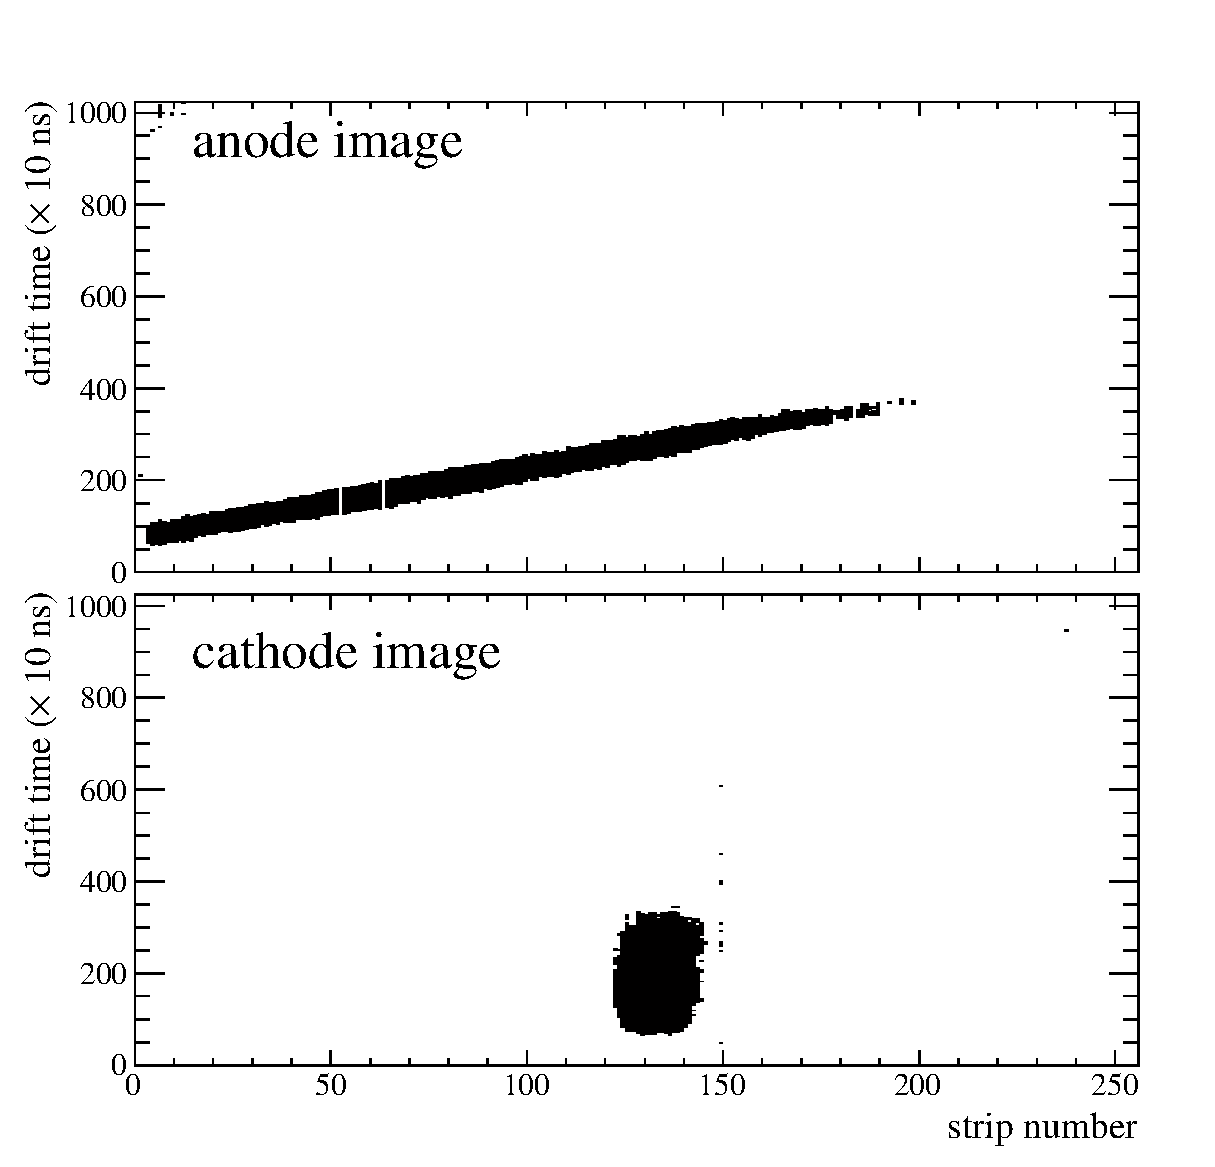
\includegraphics[clip, width=\columnwidth, trim=0 0 50 0]{0211_4.eps}
    \caption{$\alpha$線源によるトラック.}
  \end{subfigure}
  \caption{低エネルギー$\alpha$粒子のトラック [\isoButaneHydro の場合].}
  \label{fig::track_ic4h10_h2_loss}
\end{figure}
\begin{figure}
  \centering
  \begin{subfigure}{0.48\columnwidth}
    \centering
    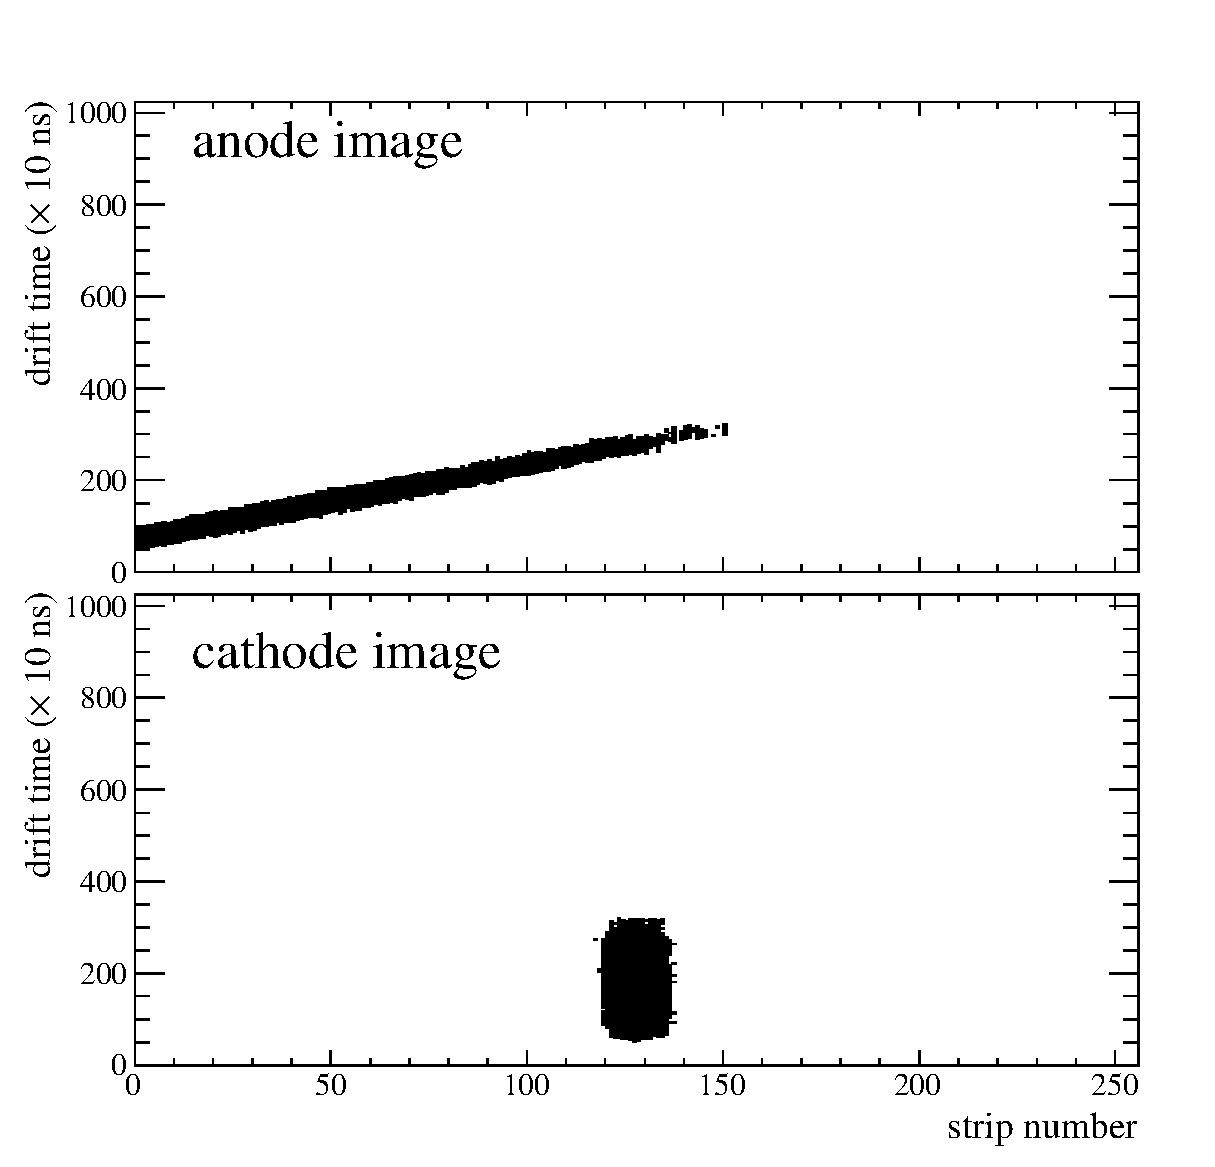
\includegraphics[clip, width=\columnwidth, trim=0 0 50 0]{a_source_iC4H10_1_He_9_100_nostr_0.eps}
    \caption{シミュレーションによるトラック.}
  \end{subfigure}
  \begin{subfigure}{0.48\columnwidth}
    \centering
    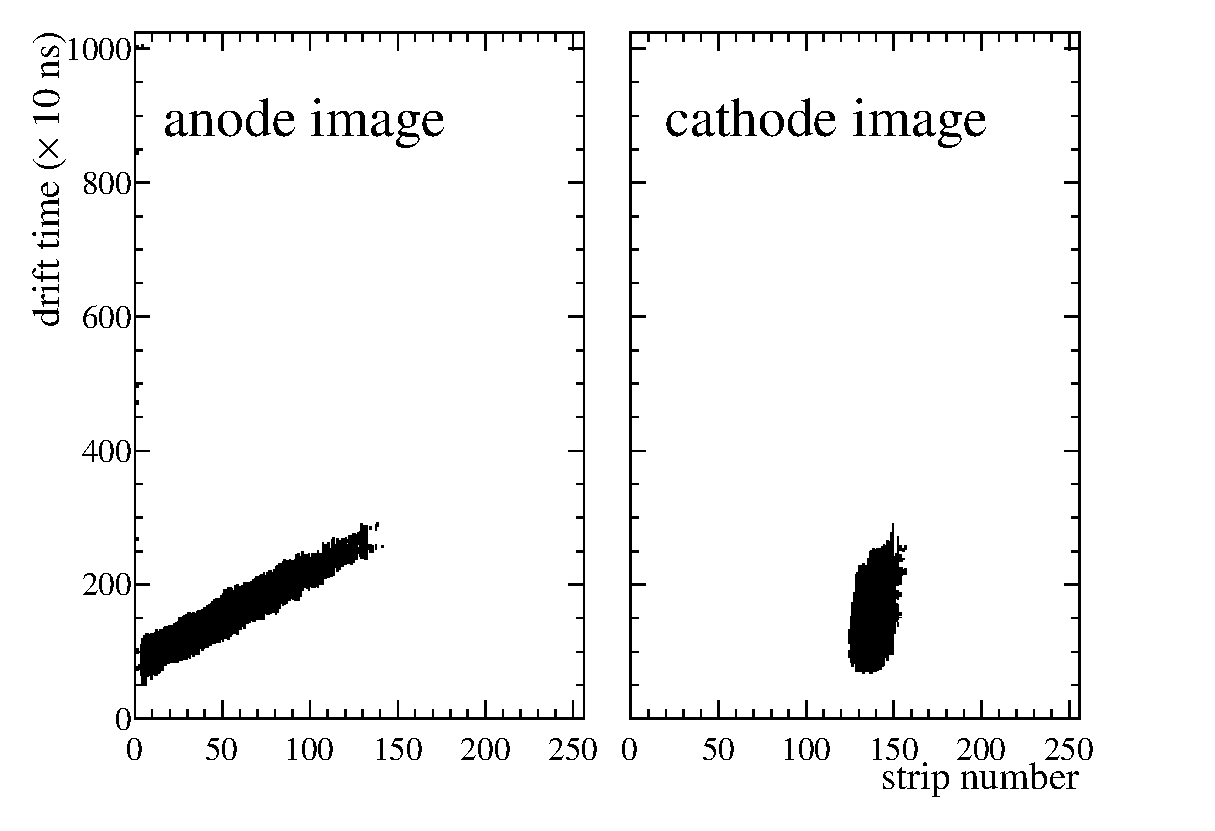
\includegraphics[clip, width=\columnwidth, trim=0 0 50 0]{0203_10.eps}
    \caption{$\alpha$線源によるトラック.}
  \end{subfigure}
  \caption{低エネルギー$\alpha$粒子のトラック [\isoButaneHerium の場合].}
  \label{fig::track_ic4h10_he_loss}
\end{figure}

\section{トリプルアルファ反応のシミュレーション}
\label{sec::triple_alpha_simulation}
$\alpha$線源から放出される$\alpha$粒子のトラックを再現することができたので,
同じ設定で${}^{12}{\mathrm{C}}({\mathrm{n}},{\mathrm{n}}')3\alpha$反応をシミュレーションによって生成した.
このシミュレーションでは以下のように3つの$\alpha$粒子を生成した.
\begin{enumerate}
\item
  ${}^{12}\mathrm{C}$を\SI{14}{\mega\electronvolt}の中性子との非弾性散乱により$0_2^+$状態に励起させる.
  この際,重心系で一様な散乱角で散乱させる.
\item
  ${}^{12}\mathrm{C} (0_2^+)$を$\alpha$粒子と${}^{8}\mathrm{Be}$に位相空間で一様に崩壊させる.
\item
  崩壊してできた${}^{8}\mathrm{Be}$を2つの$\alpha$粒子へ位相空間で一様に崩壊させる.
\end{enumerate}
このようにして得た$\alpha$粒子のトラックを生成する.
トラックの生成方法は前節で述べた通りである.
生成したトラックの例を
図\ref{fig::three_alpha_ch4} [\Methane~(\SI{50}{\hecto\pascal})],
\ref{fig::three_alpha_ch4_h2} [\Methane~(\SI{100}{\hecto\pascal})],
\ref{fig::three_alpha_ch4_he} [\Methane~(\SI{100}{\hecto\pascal})],
\ref{fig::three_alpha_ic4h10_h2} [\isoButaneHydro~(\SI{100}{\hecto\pascal})],
\ref{fig::three_alpha_ic4h10_he} [\isoButaneHerium~(\SI{100}{\hecto\pascal})] に示す.
ここでは,3つのトラックを確認できたイベントを示した.
生成されたイベントの中には$\alpha$粒子のエネルギーと放出角度によっては,
3本のトラックを個別に確認できないイベントも含まれている.
図\ref{fig::not_three_alpha_ch4} [\Methane~(\SI{50}{\hecto\pascal})],
\ref{fig::not_three_alpha_ch4_h2} [\MethaneHydro~(\SI{100}{\hecto\pascal})],
\ref{fig::not_three_alpha_ch4_he} [\MethaneHerium~(\SI{100}{\hecto\pascal})],
\ref{fig::not_three_alpha_ic4h10_h2} [\isoButaneHydro~(\SI{100}{\hecto\pascal})],
\ref{fig::not_three_alpha_ic4h10_he} [\isoButaneHerium~(\SI{100}{\hecto\pascal})] に
2本しかトラックを確認できないイベントの例を示す.

\begin{figure}
  \centering
  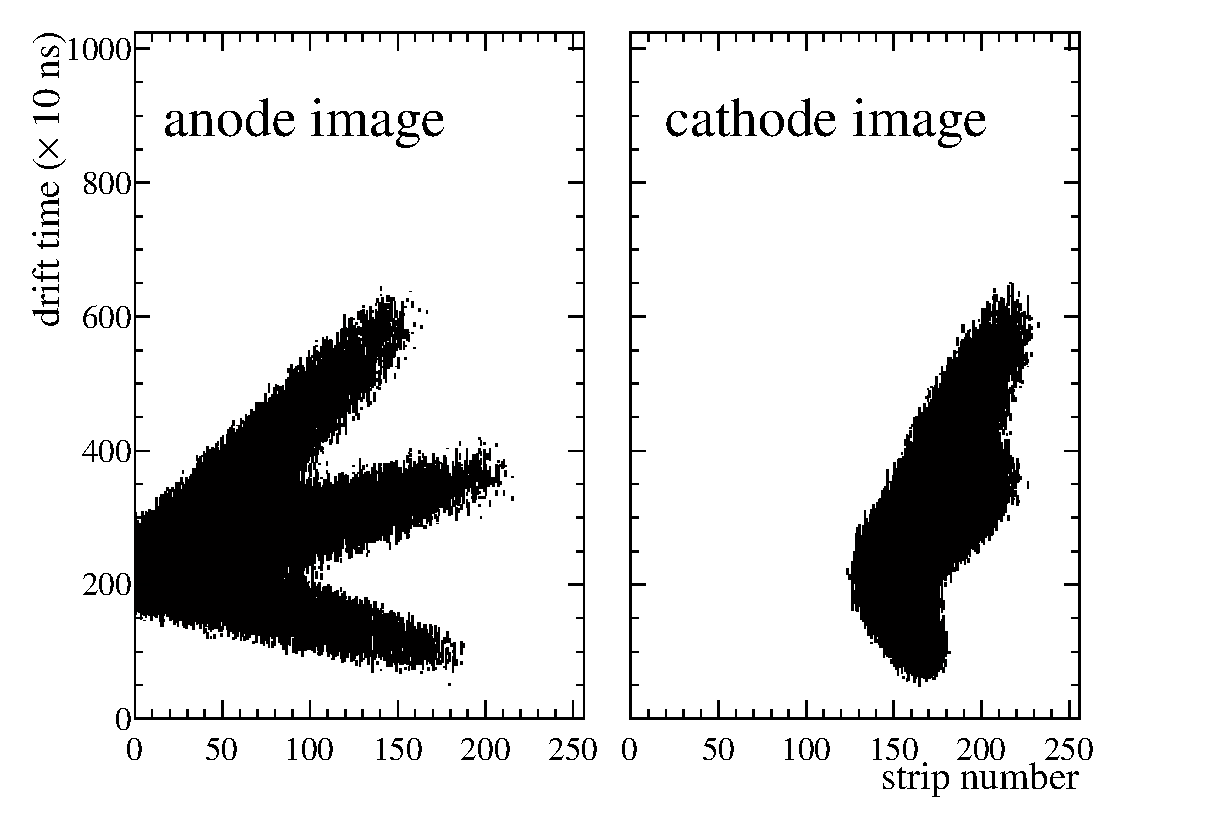
\includegraphics[clip, width=0.8\columnwidth]{10020_7.eps}
  \caption{3$\alpha$のシミュレーション画像 [\Methane の場合].}
  \label{fig::three_alpha_ch4}
\end{figure}

\begin{figure}
  \centering
  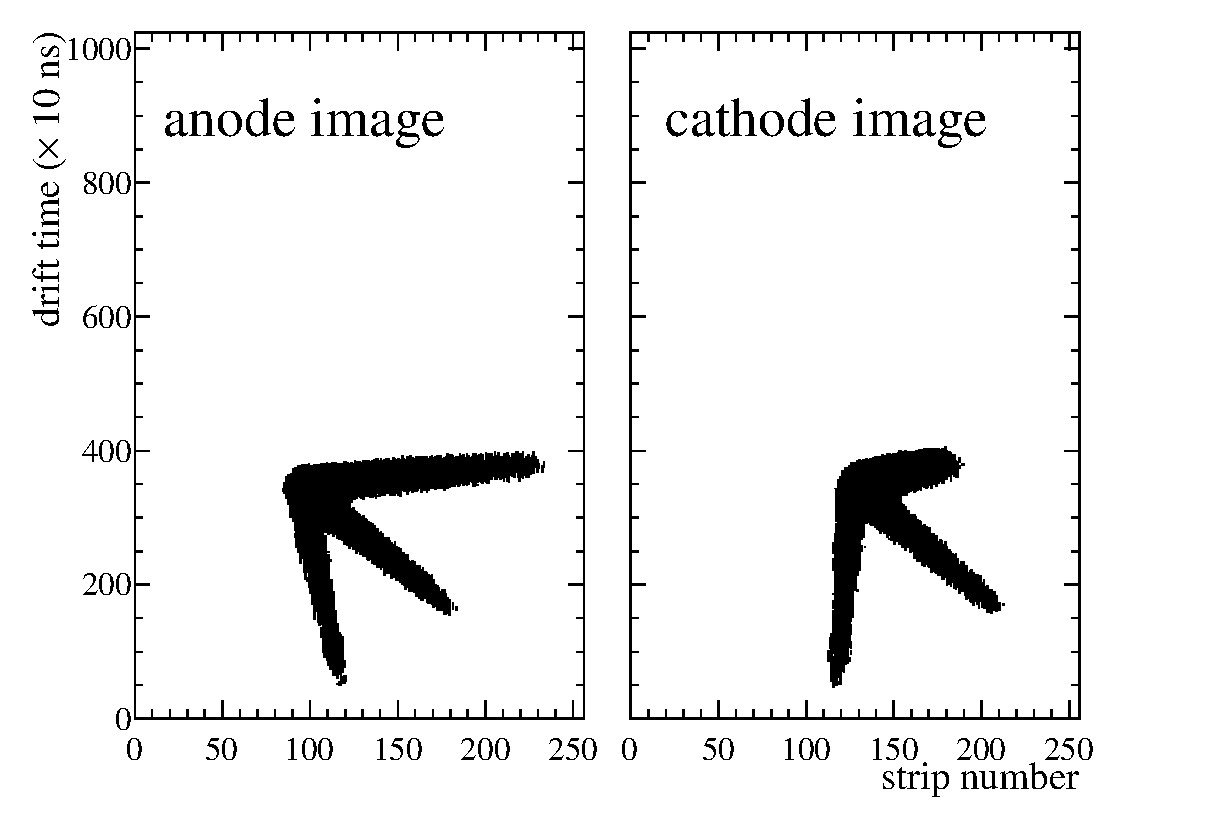
\includegraphics[clip, width=0.8\columnwidth]{10022_15.eps}
  \caption{3$\alpha$のシミュレーション画像 [\MethaneHydro の場合].}
  \label{fig::three_alpha_ch4_h2}
\end{figure}

\begin{figure}
  \centering
  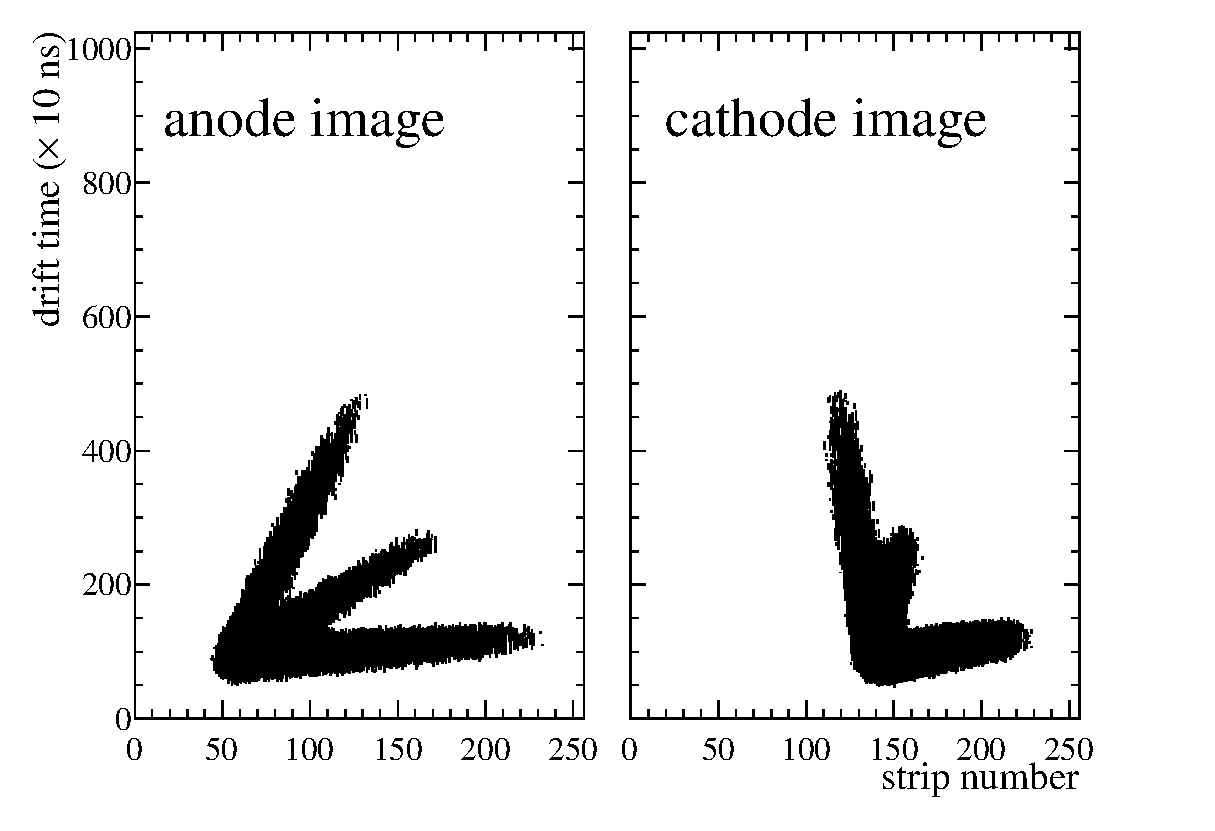
\includegraphics[clip, width=0.8\columnwidth]{10021_5.eps}
  \caption{3$\alpha$のシミュレーション画像 [\MethaneHerium の場合].}
  \label{fig::three_alpha_ch4_he}
\end{figure}

\begin{figure}
  \centering
  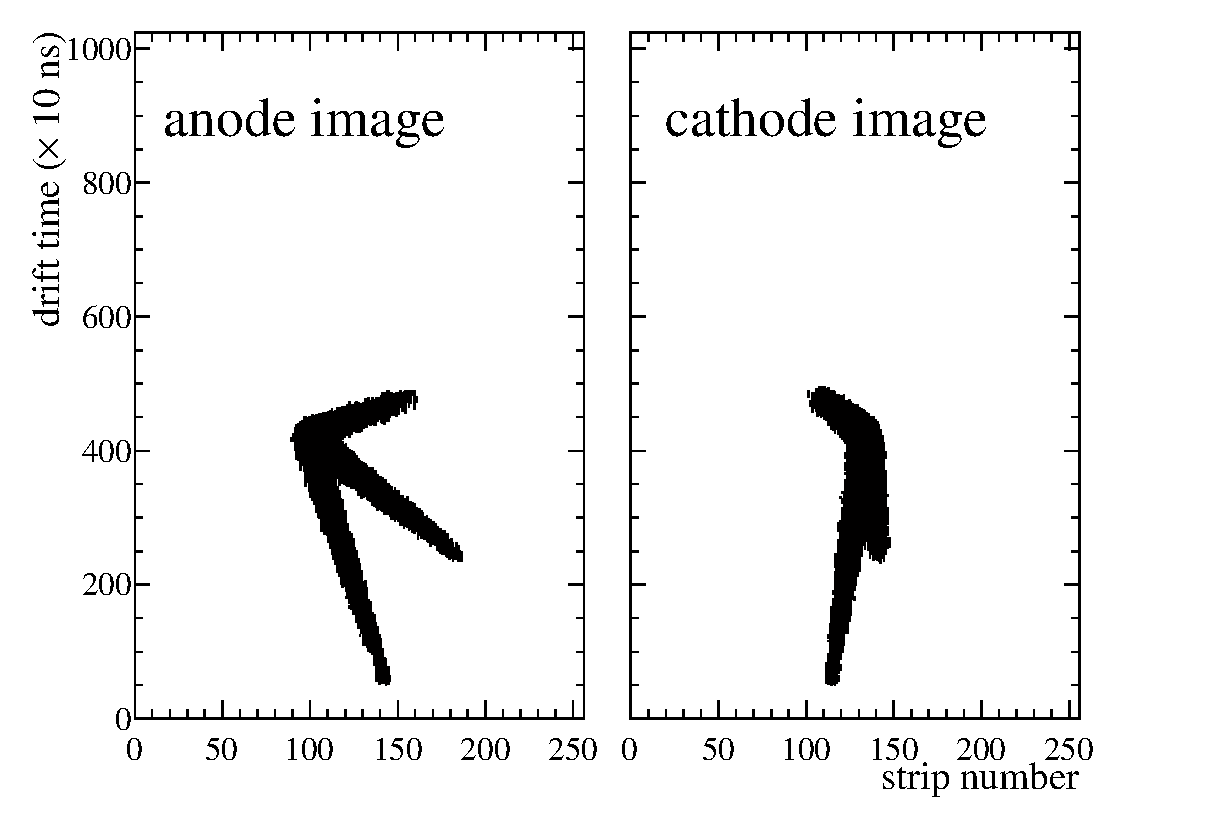
\includegraphics[clip, width=0.8\columnwidth]{10024_9.eps}
  \caption{3$\alpha$のシミュレーション画像 [\isoButaneHydro の場合].}
  \label{fig::three_alpha_ic4h10_h2}
\end{figure}

\begin{figure}
  \centering
  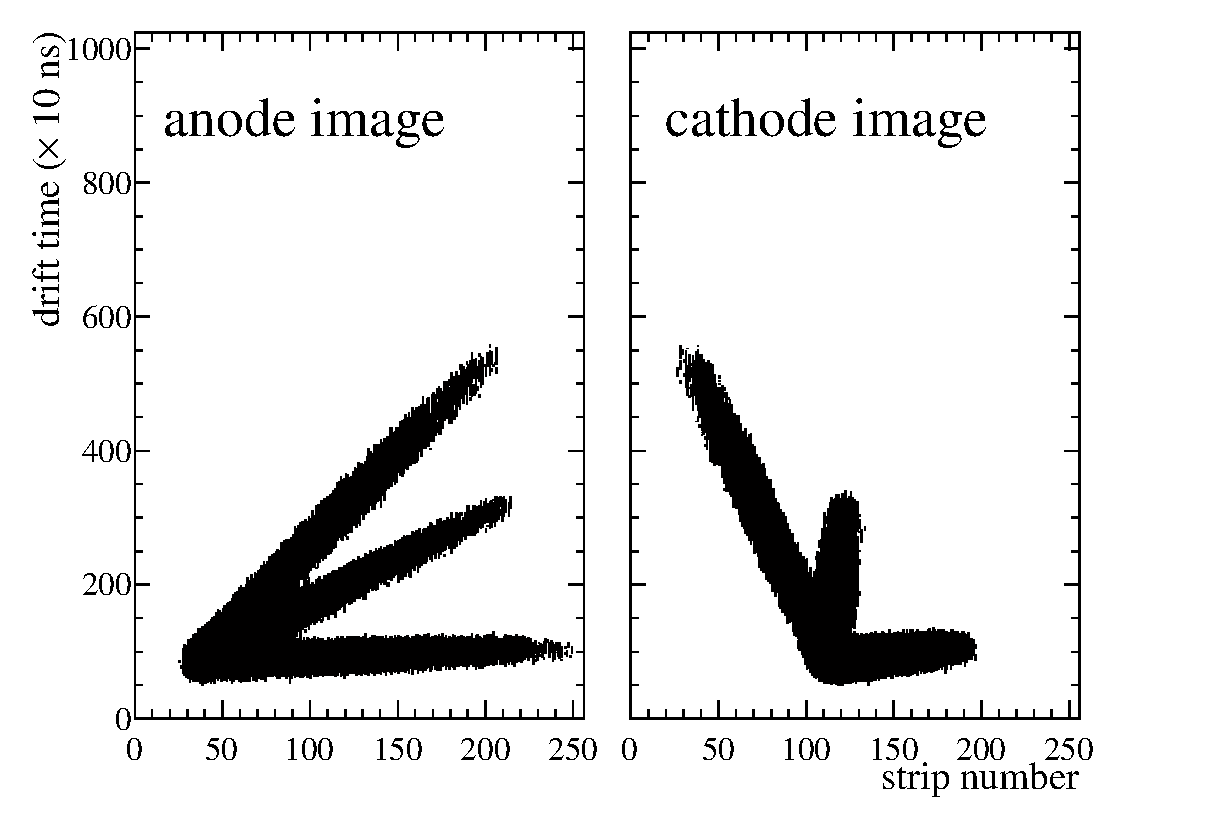
\includegraphics[clip, width=0.8\columnwidth]{10023_0.eps}
  \caption{3$\alpha$のシミュレーション画像 [\isoButaneHerium の場合].}
  \label{fig::three_alpha_ic4h10_he}
\end{figure}
\begin{figure}
  \centering
  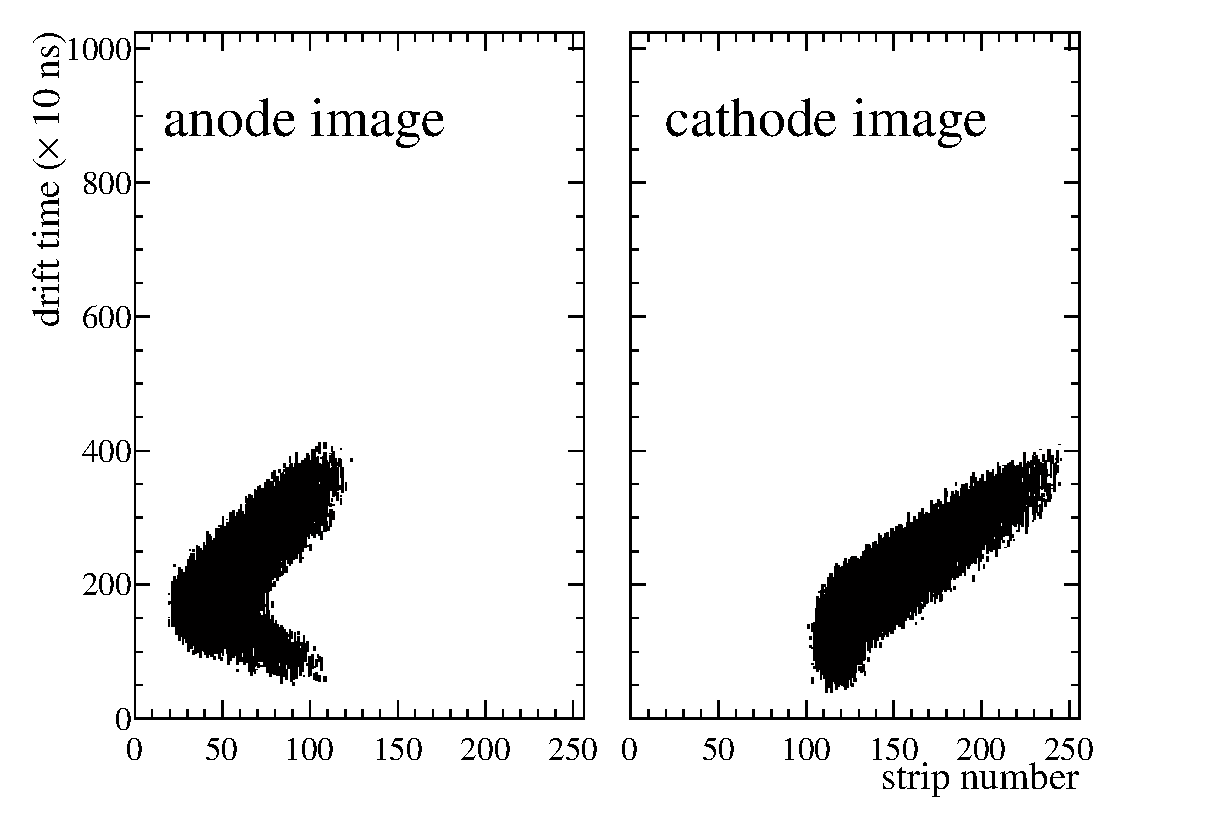
\includegraphics[clip, width=0.8\columnwidth]{10020_5.eps}
  \caption{2本しかトラックを確認できないイベントの画像 [\Methane の場合].}
  \label{fig::not_three_alpha_ch4}
\end{figure}
\begin{figure}
  \centering
  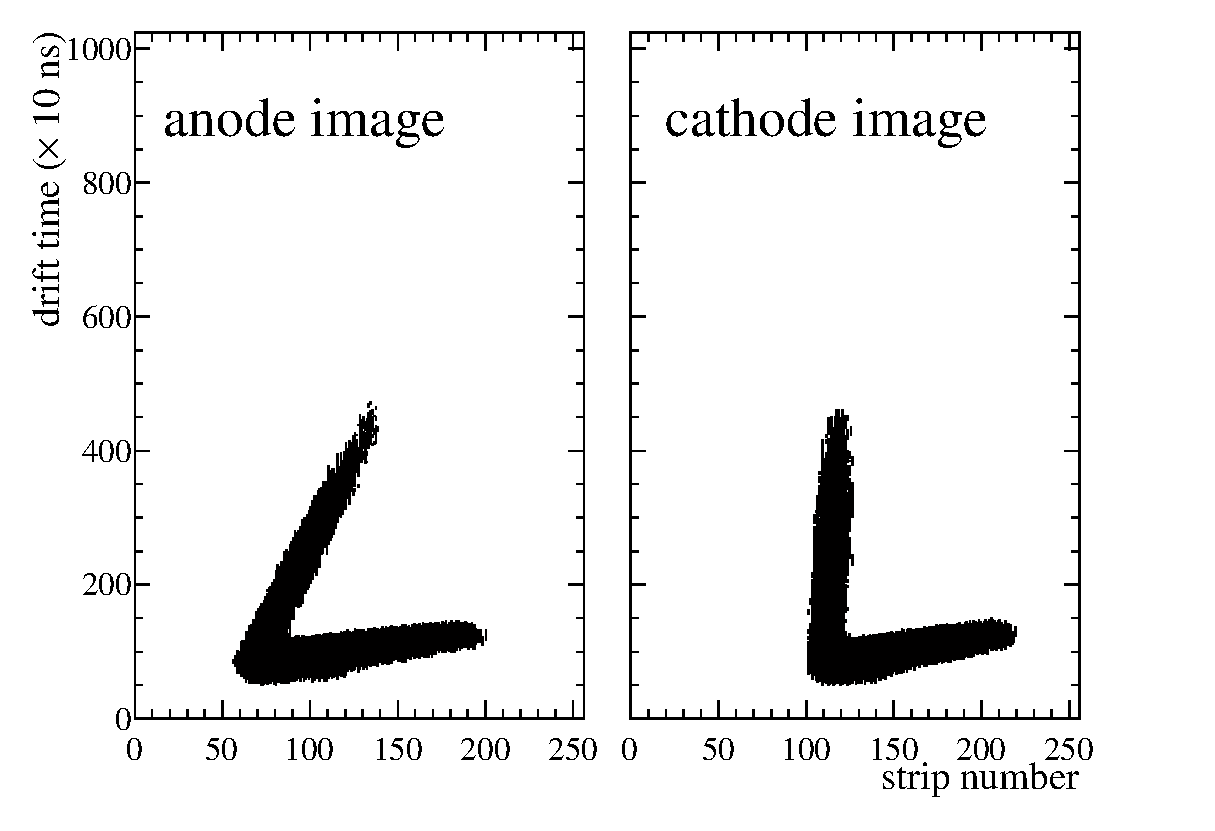
\includegraphics[clip, width=0.8\columnwidth]{10022_49.eps}
  \caption{2本しかトラックを確認できないイベントの画像 [\MethaneHydro の場合].}
  \label{fig::not_three_alpha_ch4_h2}
\end{figure}
\begin{figure}
  \centering
  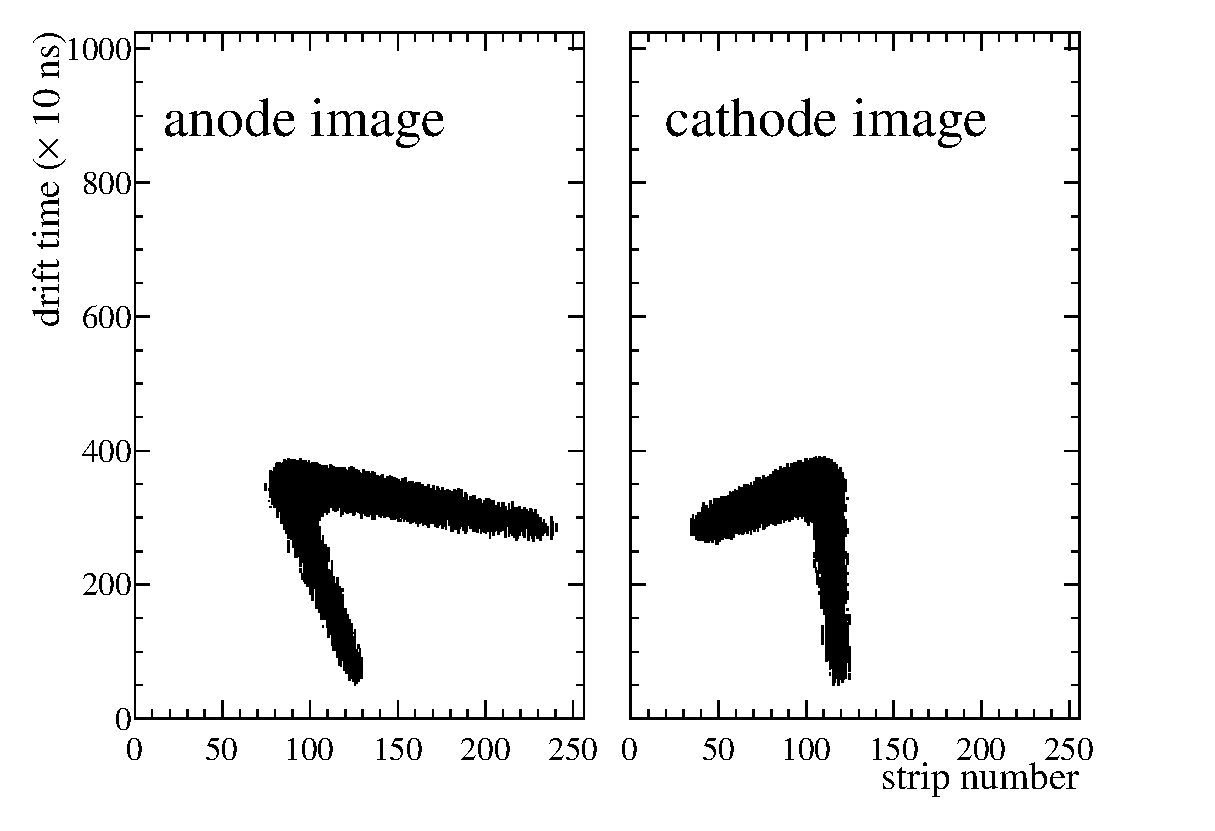
\includegraphics[clip, width=0.8\columnwidth]{10021_24.eps}
  \caption{2本しかトラックを確認できないイベントの画像 [\MethaneHerium の場合].}
  \label{fig::not_three_alpha_ch4_he}
\end{figure}
\begin{figure}
  \centering
  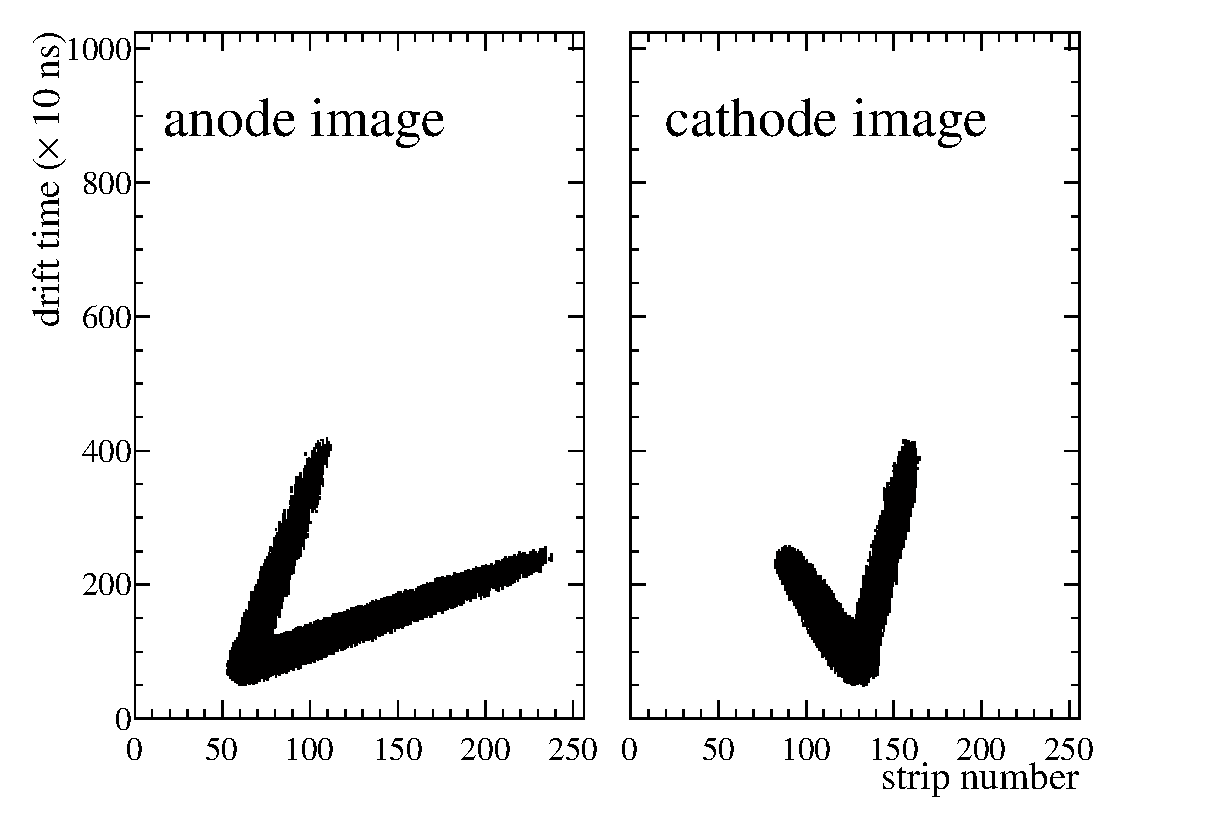
\includegraphics[clip, width=0.8\columnwidth]{10024_25.eps}
  \caption{2本しかトラックを確認できないイベントの画像 [\isoButaneHydro の場合].}
  \label{fig::not_three_alpha_ic4h10_h2}
\end{figure}
\begin{figure}
  \centering
  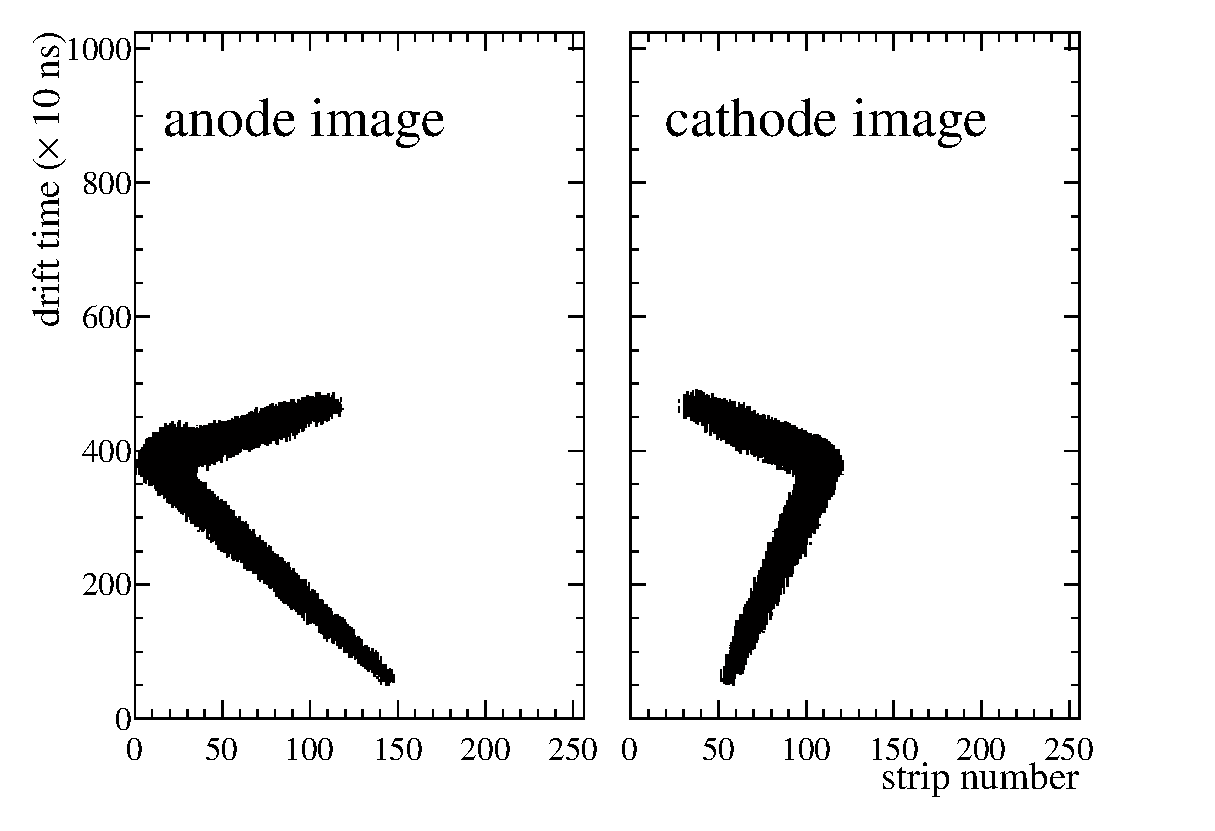
\includegraphics[clip, width=0.8\columnwidth]{10023_32.eps}
  \caption{2本しかトラックを確認できないイベントの画像 [\isoButaneHerium の場合].}
  \label{fig::not_three_alpha_ic4h10_he}
\end{figure}

\end{document}
